\documentclass[a4paper]{article}

\def\doctitle{实验四十\ 光信息处理}

\def\docabstract{光学信息处理(optical information proces-sing)是运用透镜的傅里叶变换效应,在图像的空间频域(傅里叶透镜的焦平面)对光学图像信号 进行滤波,提取或加强所需的图像(信号),滤掉或抑制不需要的图像(噪声),并进行透镜傅里叶逆变换输出处理后的图像的全部过程。光学信息处理是在傅里叶光学的基础上发展起来的。傅里叶光学的核心,在于运用透镜或其他器件产生二维图像的空间频谱,从而在频域对光信号进行处理。这次实验会对阿贝成像原理进行探究,然后利用空间滤波的方法进行观察。}

\def\dockeywords{傅立叶光学、阿贝成像原理、空间滤波}

\usepackage{see-exp}

\def\doctoc{false}

\begin{document}

%title
\input{../../texmf/see-exp-title.tex}

%contents here
\linespread{1.4} \selectfont
\section{实验概要}
\subsection{实验目的}
\hspace{2em}本实验旨在引导学生通过实验学习光学傅里叶变换以及空间频率、空间频谱和空间滤波等相关概念,探究光学成像和光学信息处理的基本原理。

%
\subsection{实验仪器}
\hspace{2em}光学平台及附件,激光器及电源,反射镜(3 个),衍射元件(2 块),扩束透镜及小孔,准直透镜(焦距为 250 mm),成像透镜(2 个,焦距均为 250 mm),成像镜头,滤波器(2块),毛玻璃,可调光阑,白屏,CCD,微机。

\subsection{实验原理}
\hspace{2em}本实验装置将搭建在一个二维光学平台上,其光路示意图如图 1 所示,按功能分成照明光、成像与滤波、观测等三个基本模块。\par

\begin{figure}[htbp]
    \centering
    \captionsetup{justification=centering,margin=2cm}
    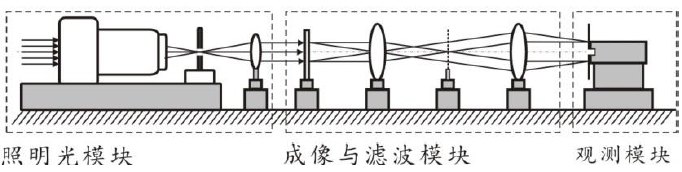
\includegraphics[width=110mm]{fig1.png}
    \caption{实验光路示意图}
\end{figure}

\hspace{2em}照明光模块用来产生照亮被观测样品的准平行光,可分别使用激光光源或白光光源。图1 的照明光模块给出的是激光光源(氦氖激光器, λ=633 nm)的情形:激光束照射在称之为“小孔滤波器”的入口处,在其出口的小孔处形成一个干净的点光源,这个点光源发出的球面波经一凸透镜(准直透镜)变成平行光。\par

\hspace{2em}成像与滤波模块是实验要探究的核心部分。图 1 所示的成像与滤波模块由两块成像透镜和处于两者之间的空间滤波器组成。对照“无限筒长”显微镜的基本结构,对着观测物的透镜称为“物镜”,另一个称为“筒镜”。将样品放置在物镜的前焦面上时,样品上各点发出的旁轴光线经物镜后变成不同的平行光,并且在物镜的后焦面上叠加出样品的空间频谱。然后,各个方向的平行光经筒镜在其后焦面上汇聚成相应的像点,呈现出样品的像。应用于光信息处理时,一对傅里叶透镜分别取代“物镜”和“筒镜”,前者做光学傅里叶正变换,后者做逆变换。应用于显微成像时,物镜实际上是固定封装的一组透镜,而筒镜仍为单凸透镜。\par

\hspace{2em}观测模块包括 CCD 相机和与之连接的计算机,用来采集和显示筒镜所成的像,也可用来采集样品的空间频谱。\par

\section{实验数据及分析}

%%%%%%%%%%%%%%%%%%%%%%%%%%%%%%%%%%%%%%%%%%%%%%%%%%%%%%%%%%%%%%%%%%%

\subsection{衍射屏上不同结构的空间频谱与像的分布}
\hspace{2em}参考图1所搭的光路,进行光学的傅里叶变换,观察并记录不同衍射屏的空间频谱和像分布。\par
\begin{figure}[H]
    \centering
    %%%%%%%%%%%%%%%%%%%%%%%%%%%%%
    \begin{subfigure}[t]{0.3\textwidth}
        \centering
        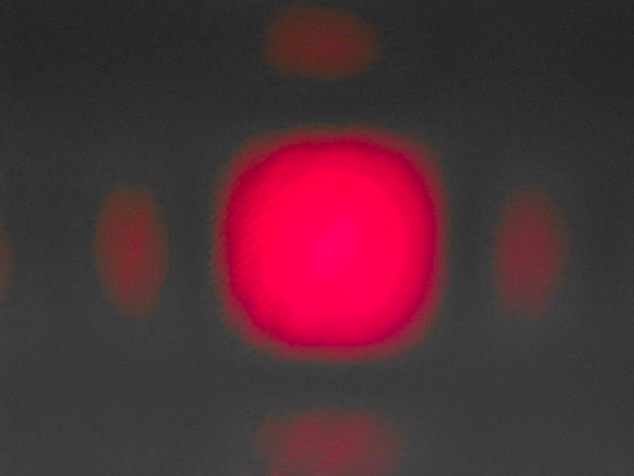
\includegraphics[width=\textwidth]{fre-done/1-1.JPG}
        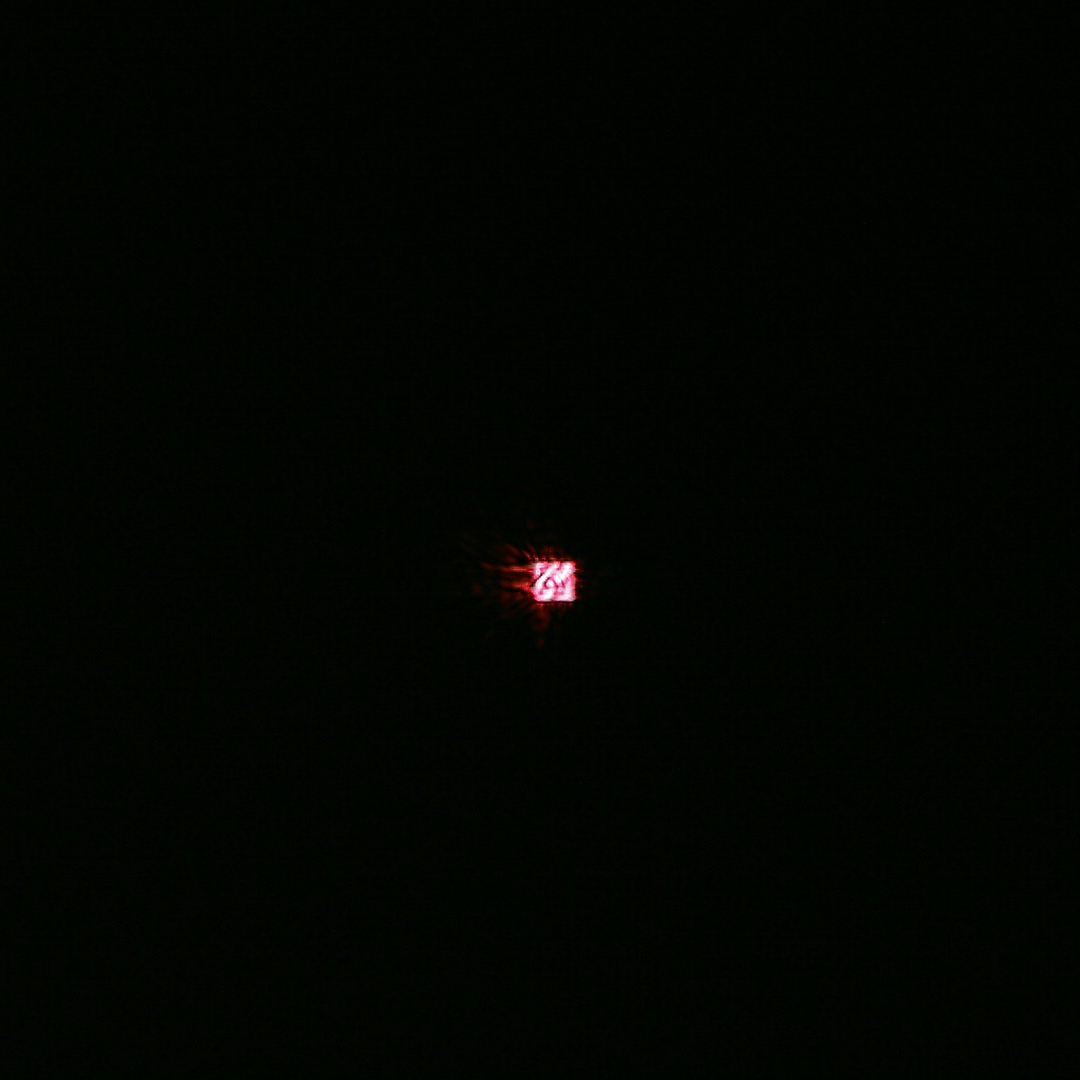
\includegraphics[width=\textwidth]{img-done/1-1.JPG}
        \captionsetup{font={normalsize,sf},justification=centering}
        \caption{单方孔}
        \label{1-1}
    \end{subfigure}
    \begin{subfigure}[t]{0.3\textwidth}
        \centering
        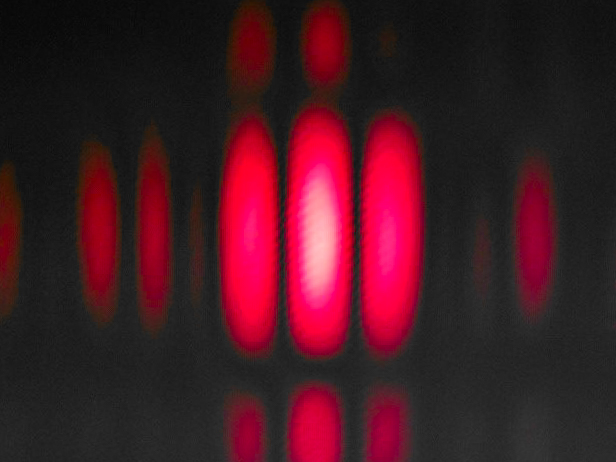
\includegraphics[width=\textwidth]{fre-done/1-2.JPG}
        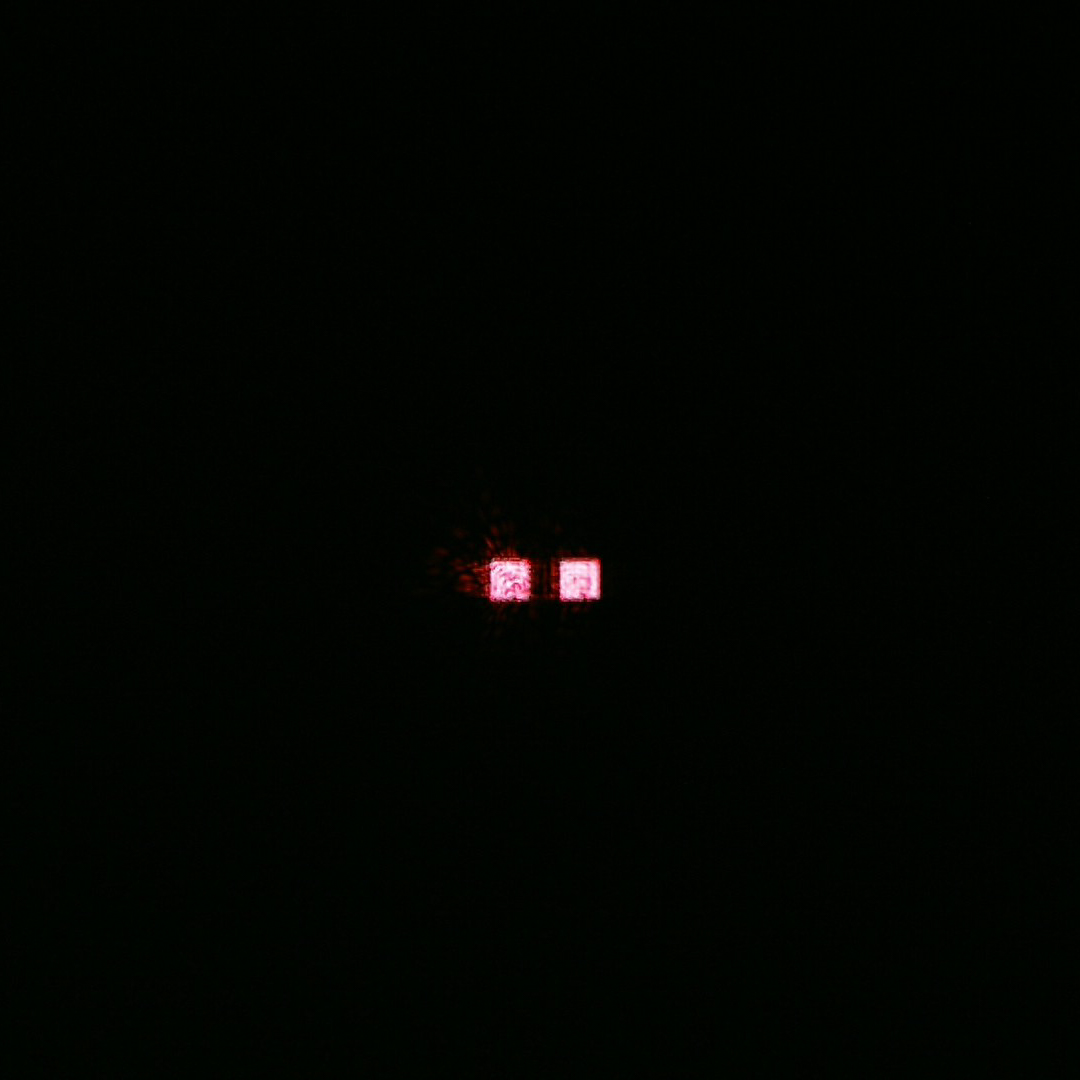
\includegraphics[width=\textwidth]{img-done/1-2.JPG}
        \captionsetup{font={normalsize,sf},justification=centering}
        \caption{双方孔}
        \label{1-2}
    \end{subfigure}
    \begin{subfigure}[t]{0.3\textwidth}
        \centering
        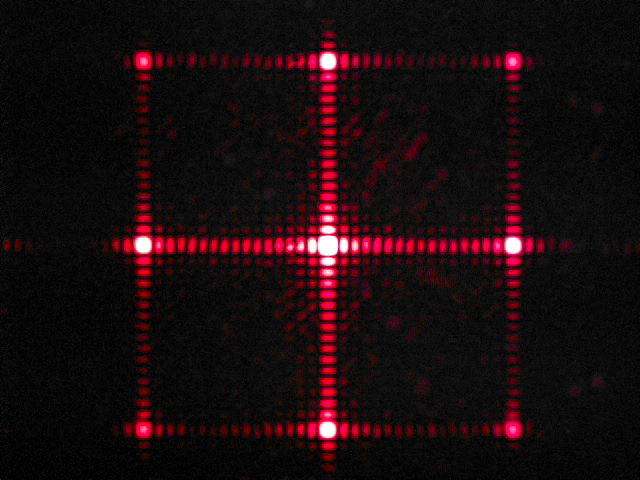
\includegraphics[width=\textwidth]{fre-done/1-3.JPG}
        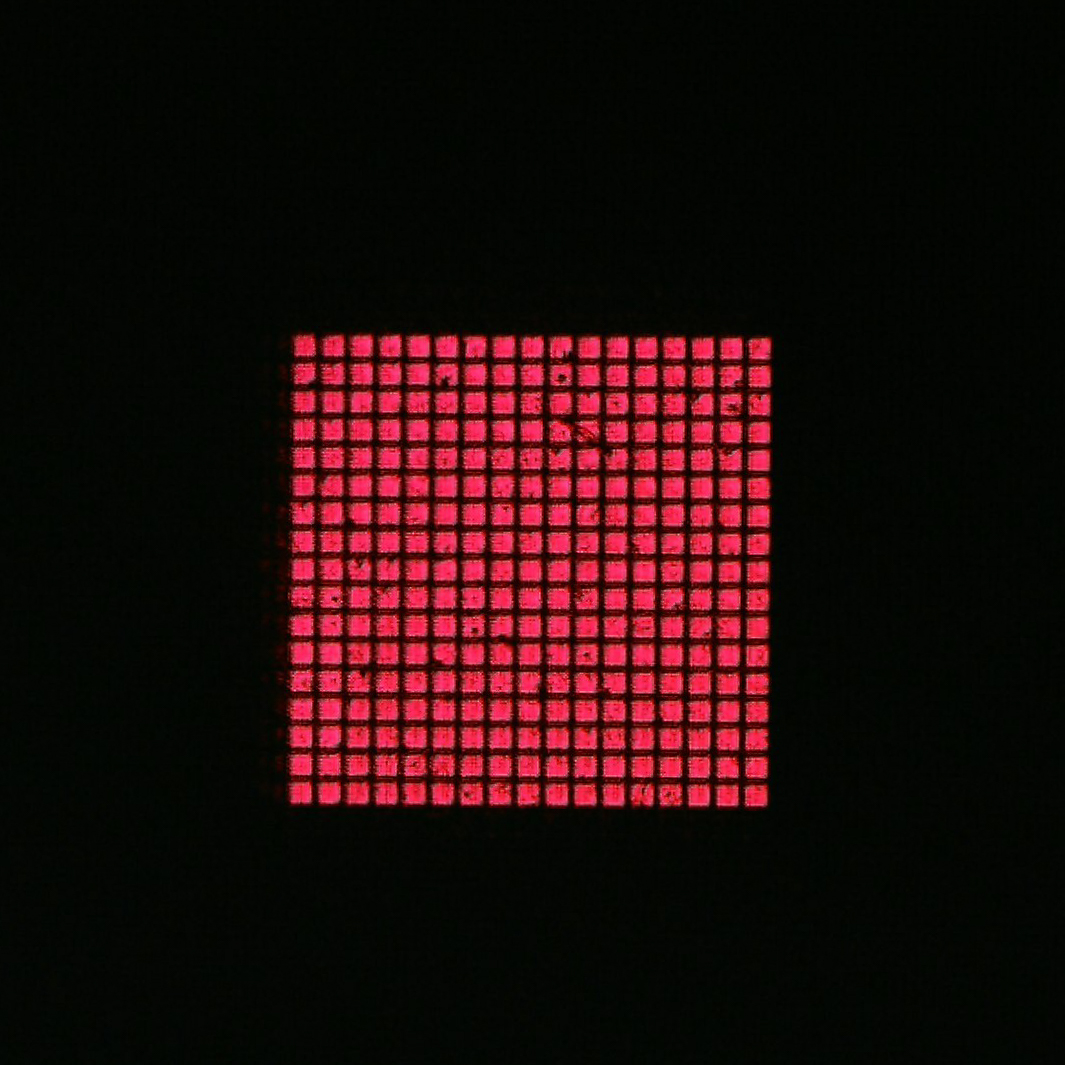
\includegraphics[width=\textwidth]{img-done/1-3.JPG}
        \captionsetup{font={normalsize,sf},justification=centering}
        \caption{方孔方阵}
        \label{1-3}
    \end{subfigure}
    %%%%%%%%%%%%%%%%%%%%%%%%%%%%%
    \begin{subfigure}[t]{0.3\textwidth}
        \centering
        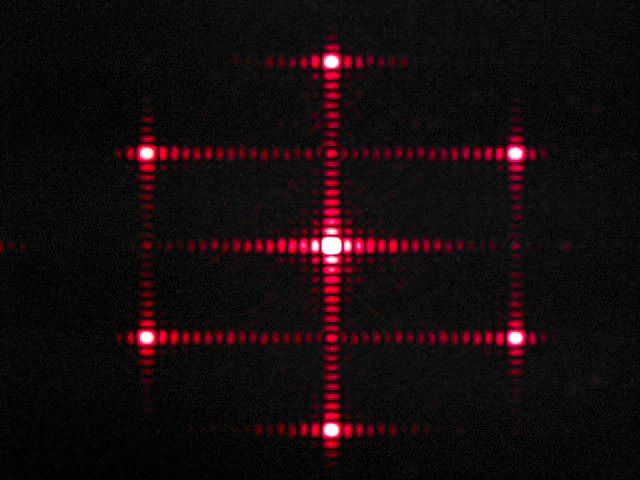
\includegraphics[width=\textwidth]{fre-done/1-4.JPG}
        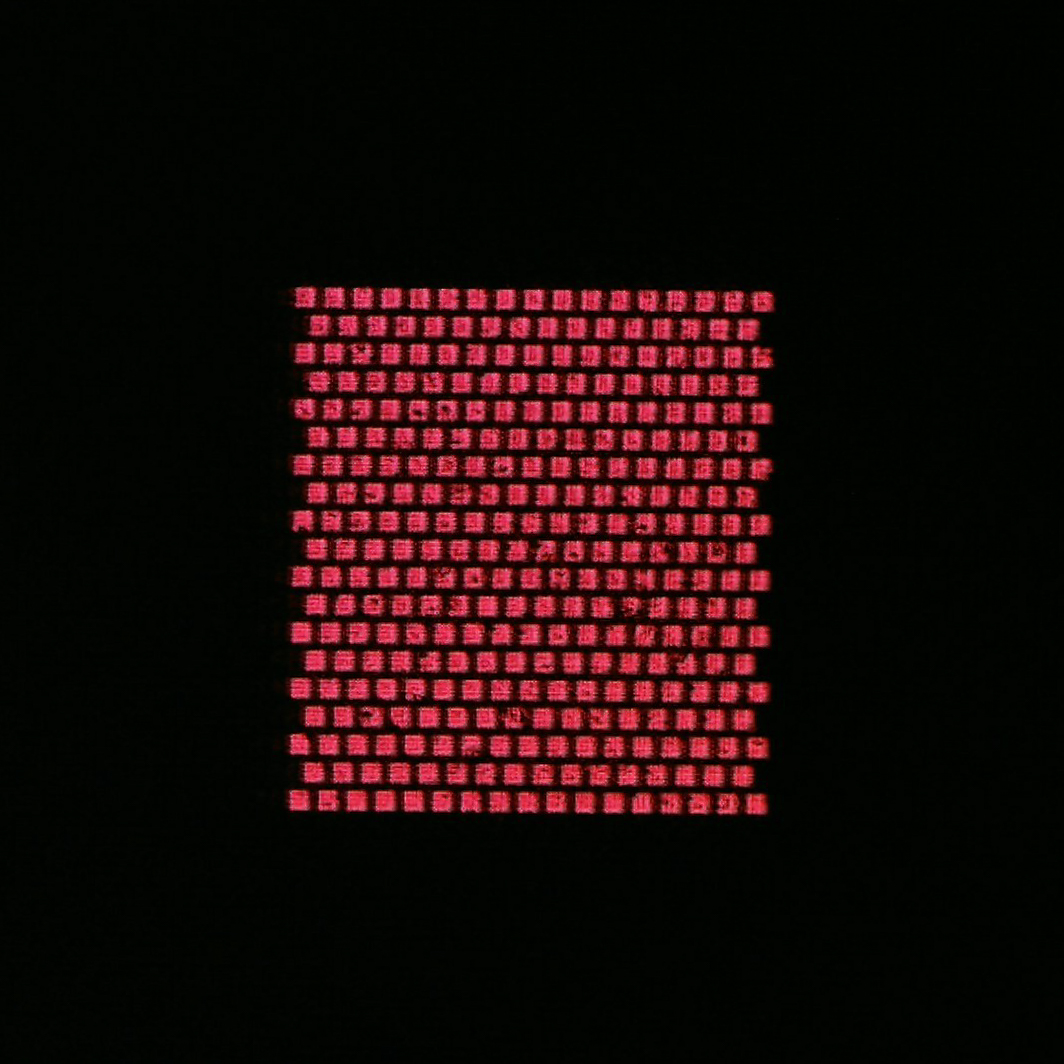
\includegraphics[width=\textwidth]{img-done/1-4.JPG}
        \captionsetup{font={normalsize,sf},justification=centering}
        \caption{方孔密排}
        \label{1-4}
    \end{subfigure}
    \begin{subfigure}[t]{0.3\textwidth}
        \centering
        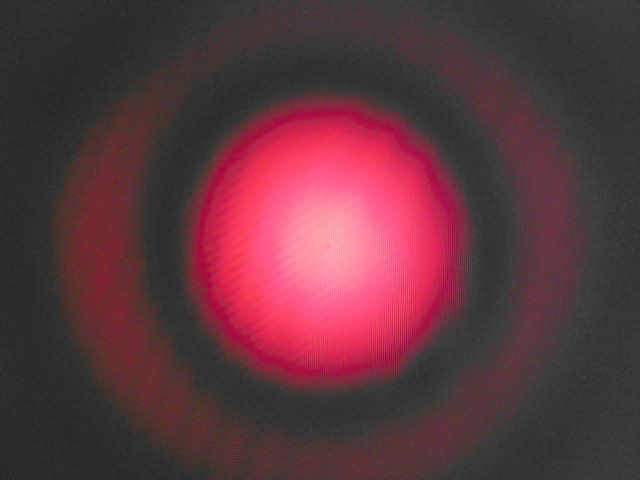
\includegraphics[width=\textwidth]{fre-done/1-5.JPG}
        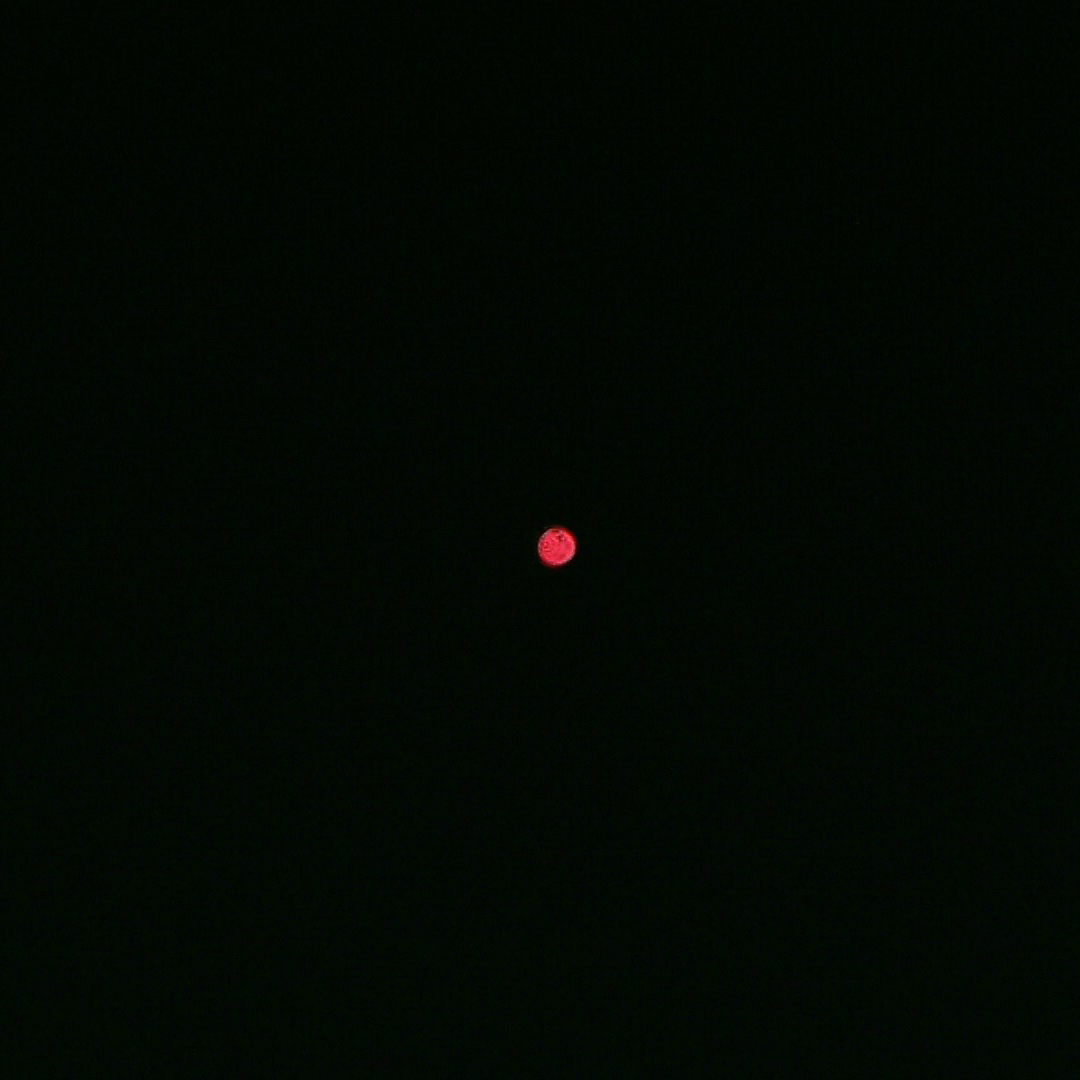
\includegraphics[width=\textwidth]{img-done/1-5.JPG}
        \captionsetup{font={normalsize,sf},justification=centering}
        \caption{单圆孔}
        \label{1-5}
    \end{subfigure}
    \begin{subfigure}[t]{0.3\textwidth}
        \centering
        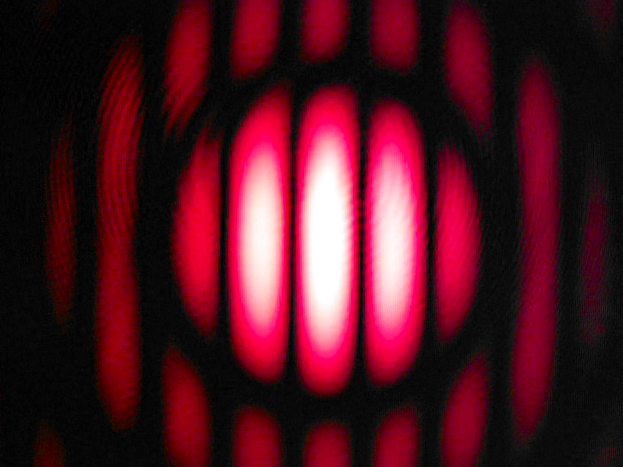
\includegraphics[width=\textwidth]{fre-done/1-6.JPG}
        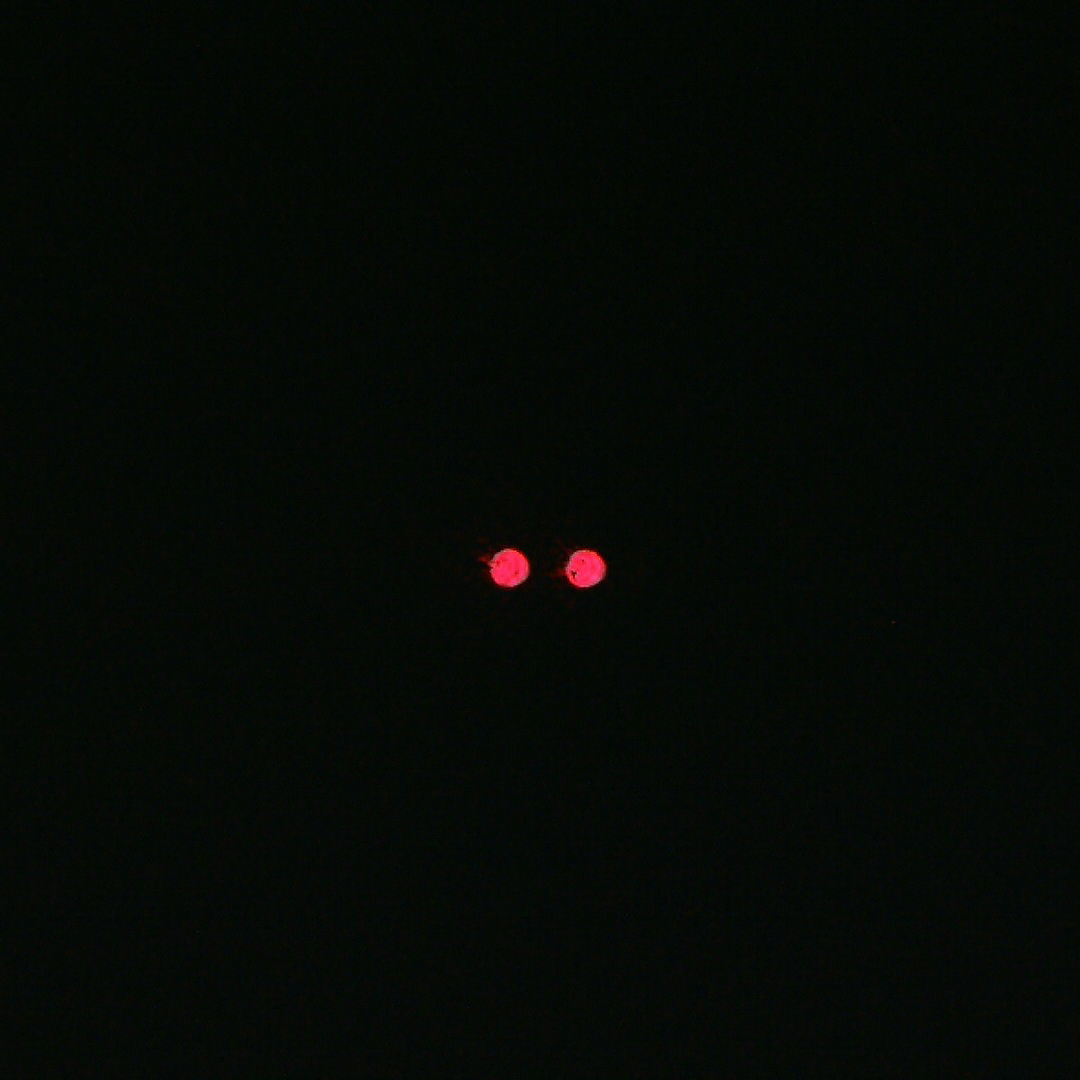
\includegraphics[width=\textwidth]{img-done/1-6.JPG}
        \captionsetup{font={normalsize,sf},justification=centering}
        \caption{双圆孔}
        \label{1-6}
    \end{subfigure}
    %%%%%%%%%%%%%%%%%%%%%%%%%%%%%
    \captionsetup{justification=centering,subrefformat=parens}
    \caption{不同屏产生的频谱与像屏上图像}

\end{figure}
\clearpage
\begin{figure}[htbp]\ContinuedFloat
    \centering
    %%%%%%%%%%%%%%%%%%%%%%%%%%%%%
    \begin{subfigure}[htbp]{0.3\textwidth}
        \centering
        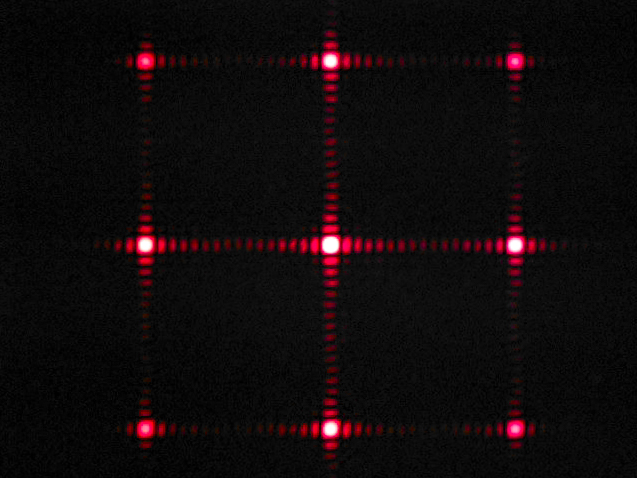
\includegraphics[width=\textwidth]{fre-done/1-7.JPG}
        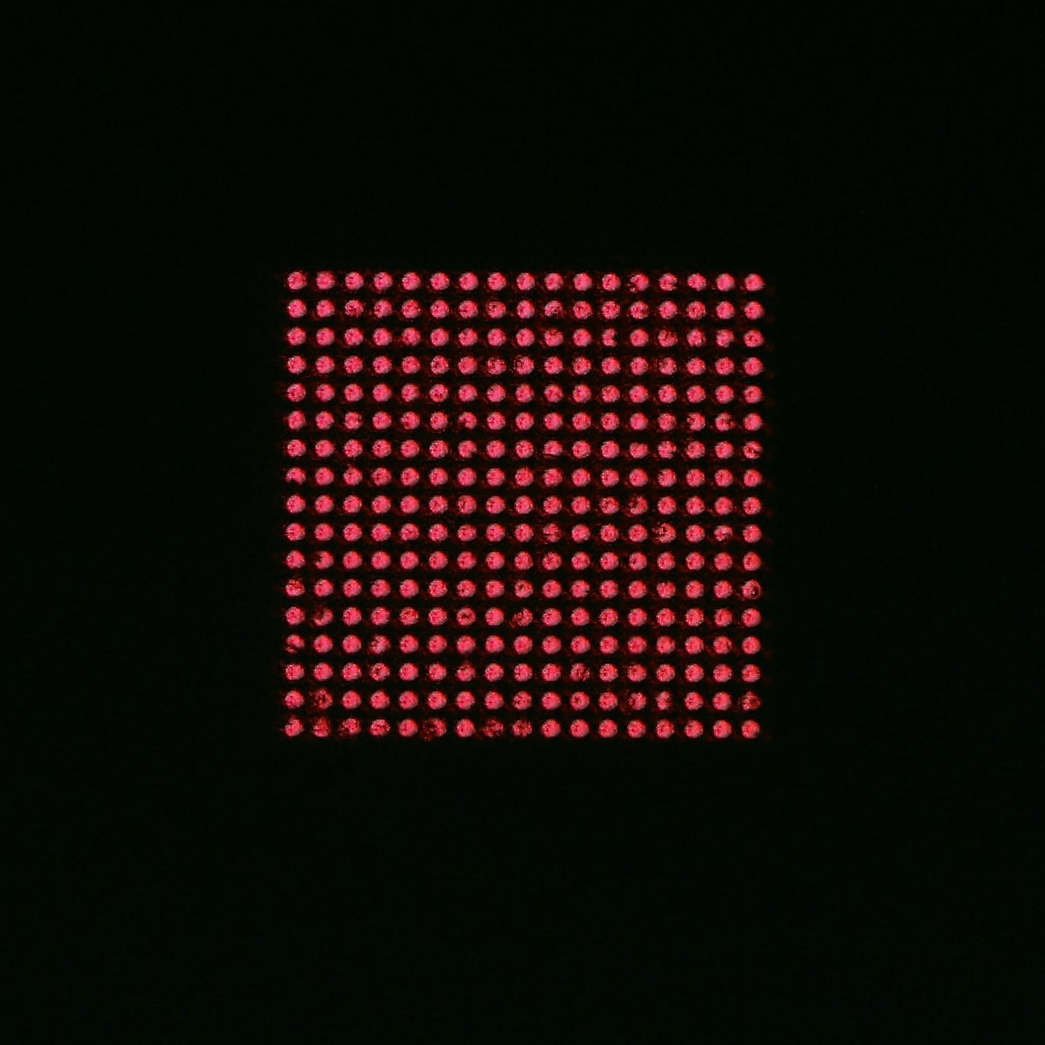
\includegraphics[width=\textwidth]{img-done/1-7.JPG}
        \captionsetup{font={normalsize,sf},justification=centering}
        \caption{圆孔方阵}
        \label{1-7}
    \end{subfigure}
    \begin{subfigure}[htbp]{0.3\textwidth}
        \centering
        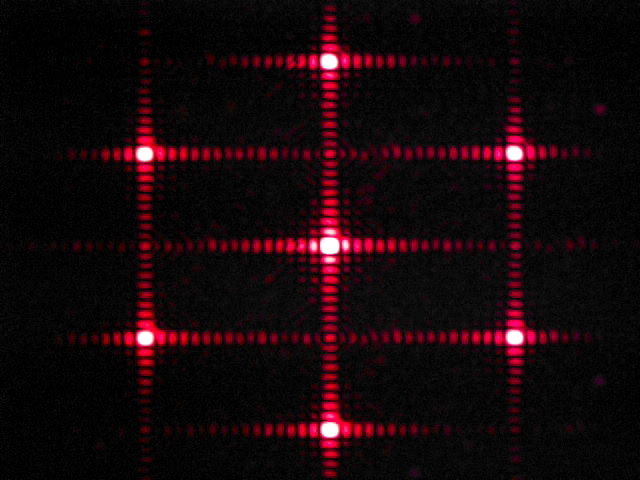
\includegraphics[width=\textwidth]{fre-done/1-8.JPG}
        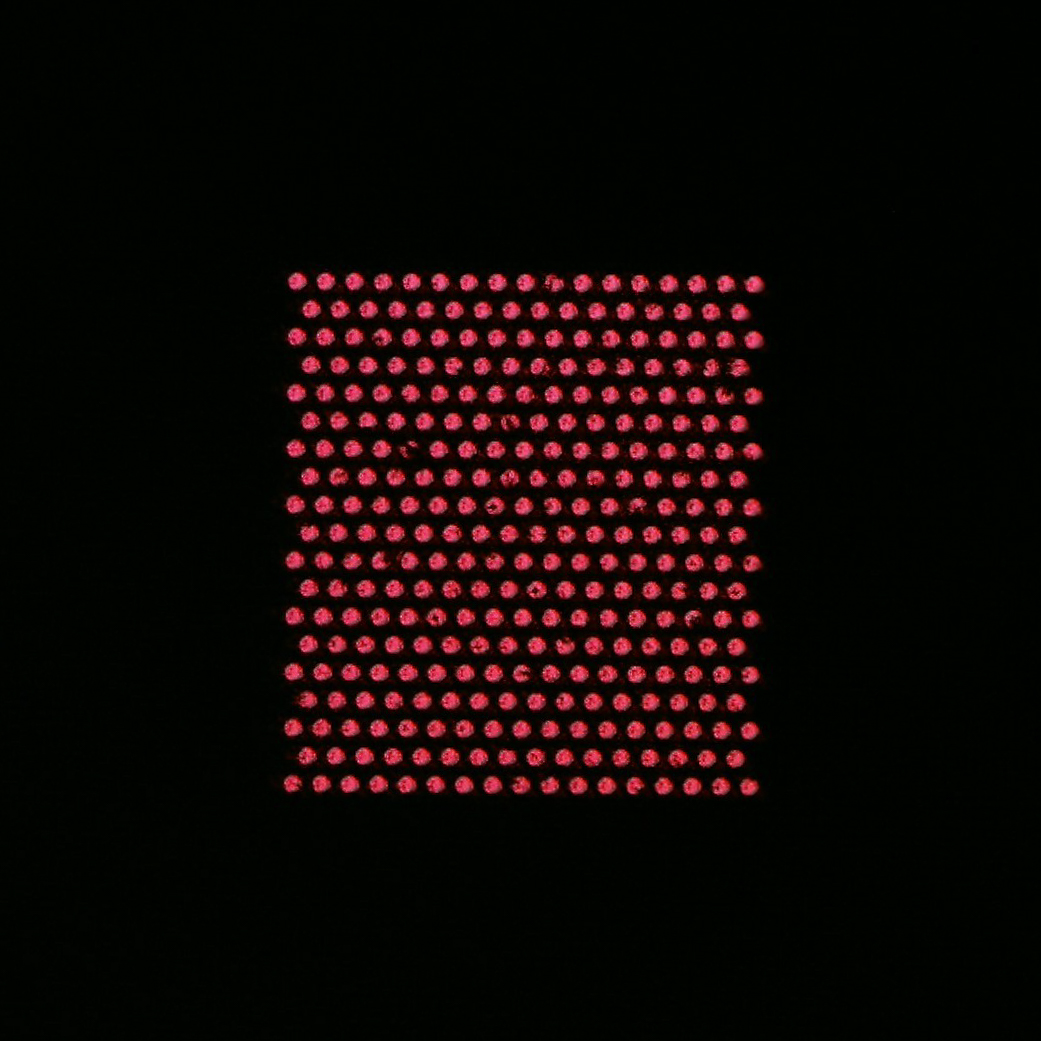
\includegraphics[width=\textwidth]{img-done/1-8.JPG}
        \captionsetup{font={normalsize,sf},justification=centering}
        \caption{圆孔密排}
        \label{1-8}
    \end{subfigure}
    \begin{subfigure}[htbp]{0.3\textwidth}
        \centering
        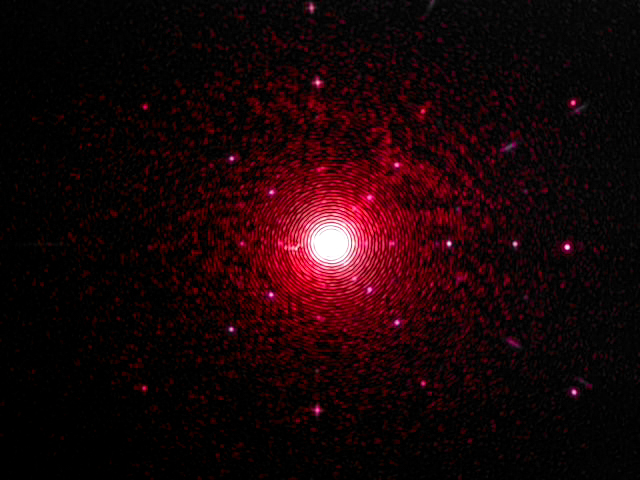
\includegraphics[width=\textwidth]{fre-done/2-1.JPG}
        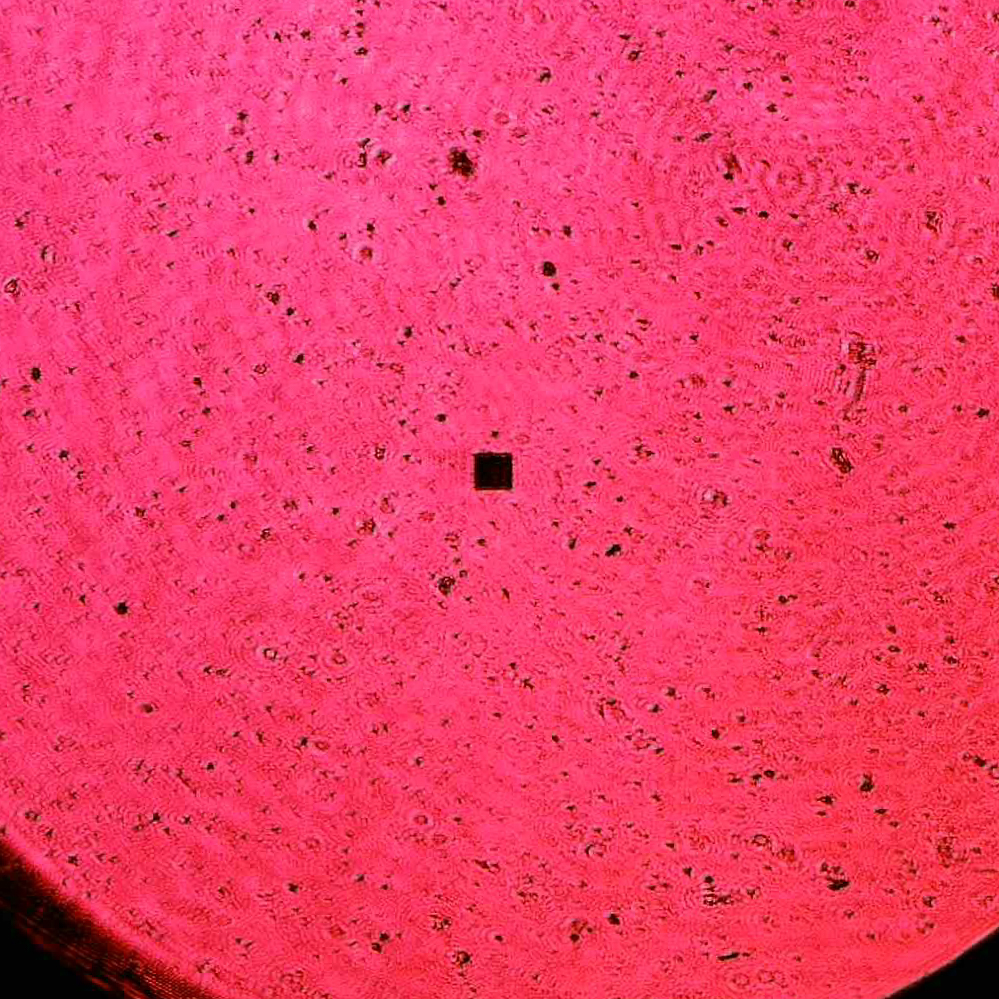
\includegraphics[width=\textwidth]{img-done/2-1.JPG}
        \captionsetup{font={normalsize,sf},justification=centering}
        \caption{单方屏}
        \label{2-1}
    \end{subfigure}
    %%%%%%%%%%%%%%%%%%%%%%%%%%%%%
    \begin{subfigure}[htbp]{0.3\textwidth}
        \centering
        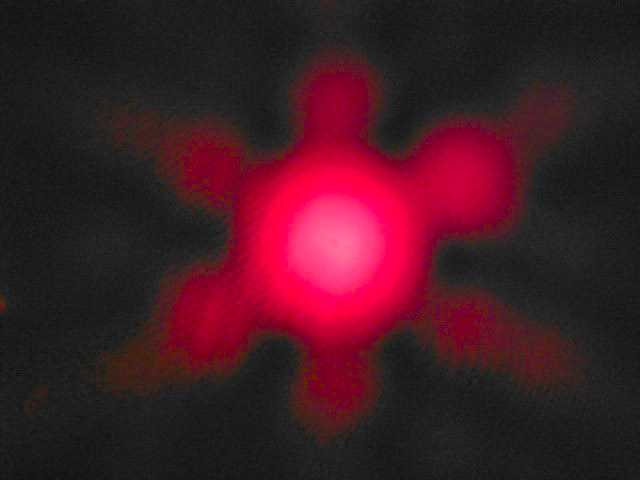
\includegraphics[width=\textwidth]{fre-done/2-2.JPG}
        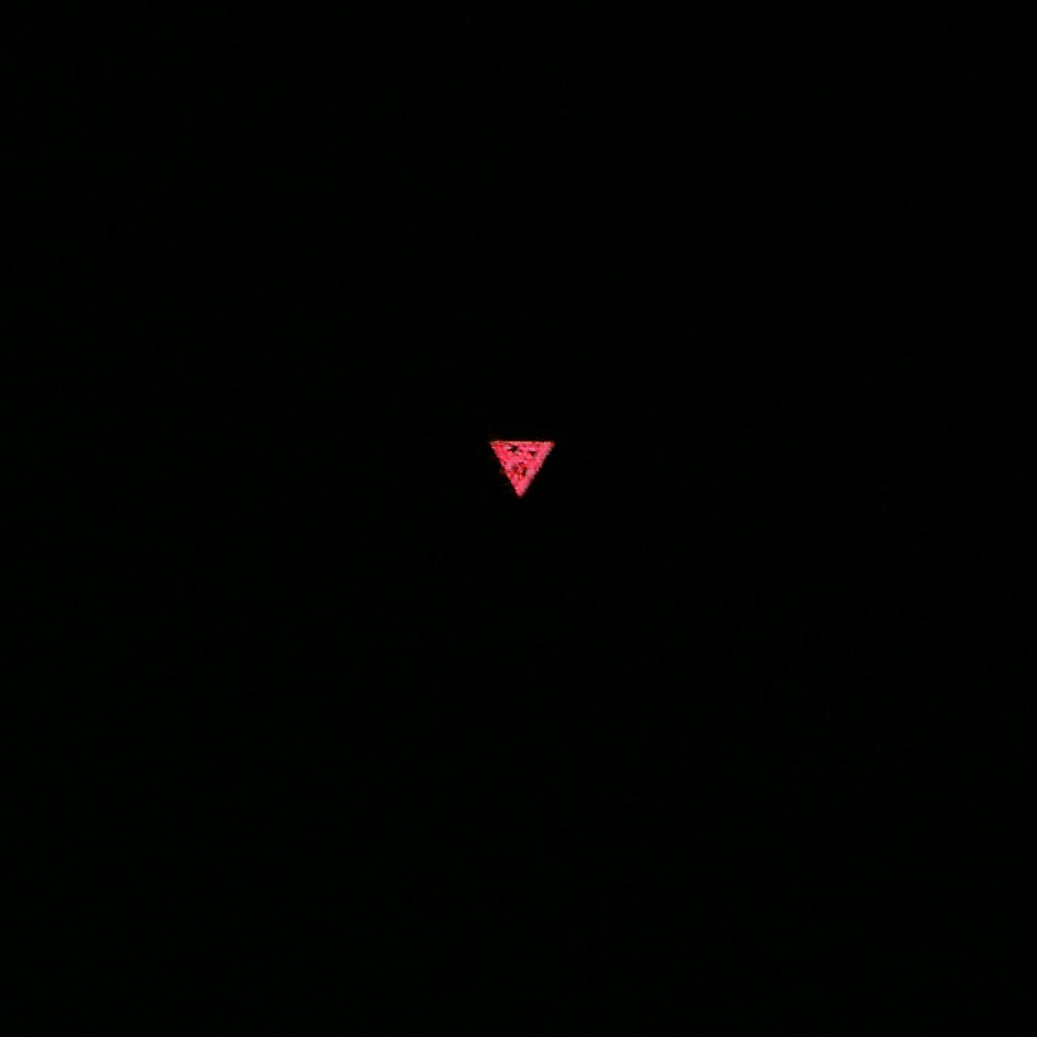
\includegraphics[width=\textwidth]{img-done/2-2.JPG}
        \captionsetup{font={normalsize,sf},justification=centering}
        \caption{等边三角孔}
        \label{2-2}
    \end{subfigure}
    \begin{subfigure}[htbp]{0.3\textwidth}
        \centering
        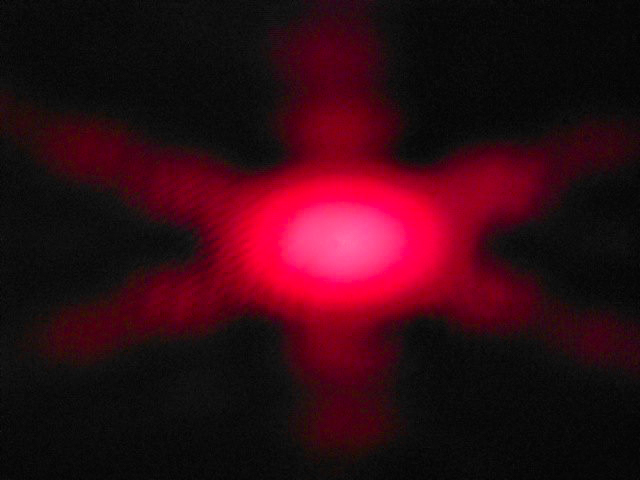
\includegraphics[width=\textwidth]{fre-done/2-3.JPG}
        
\includegraphics[width=\textwidth]{img-done/2-3.JPG}
        \captionsetup{font={normalsize,sf},justification=centering}
        \caption{等腰三角孔}
        \label{2-3}
    \end{subfigure}
    \begin{subfigure}[htbp]{0.3\textwidth}
        \centering
        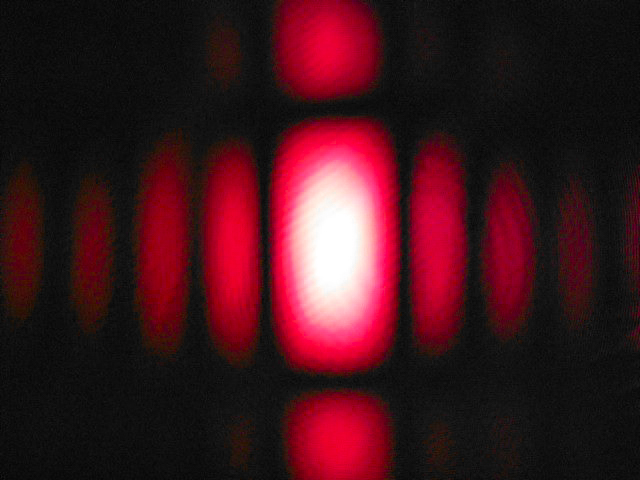
\includegraphics[width=\textwidth]{fre-done/2-4.JPG}
        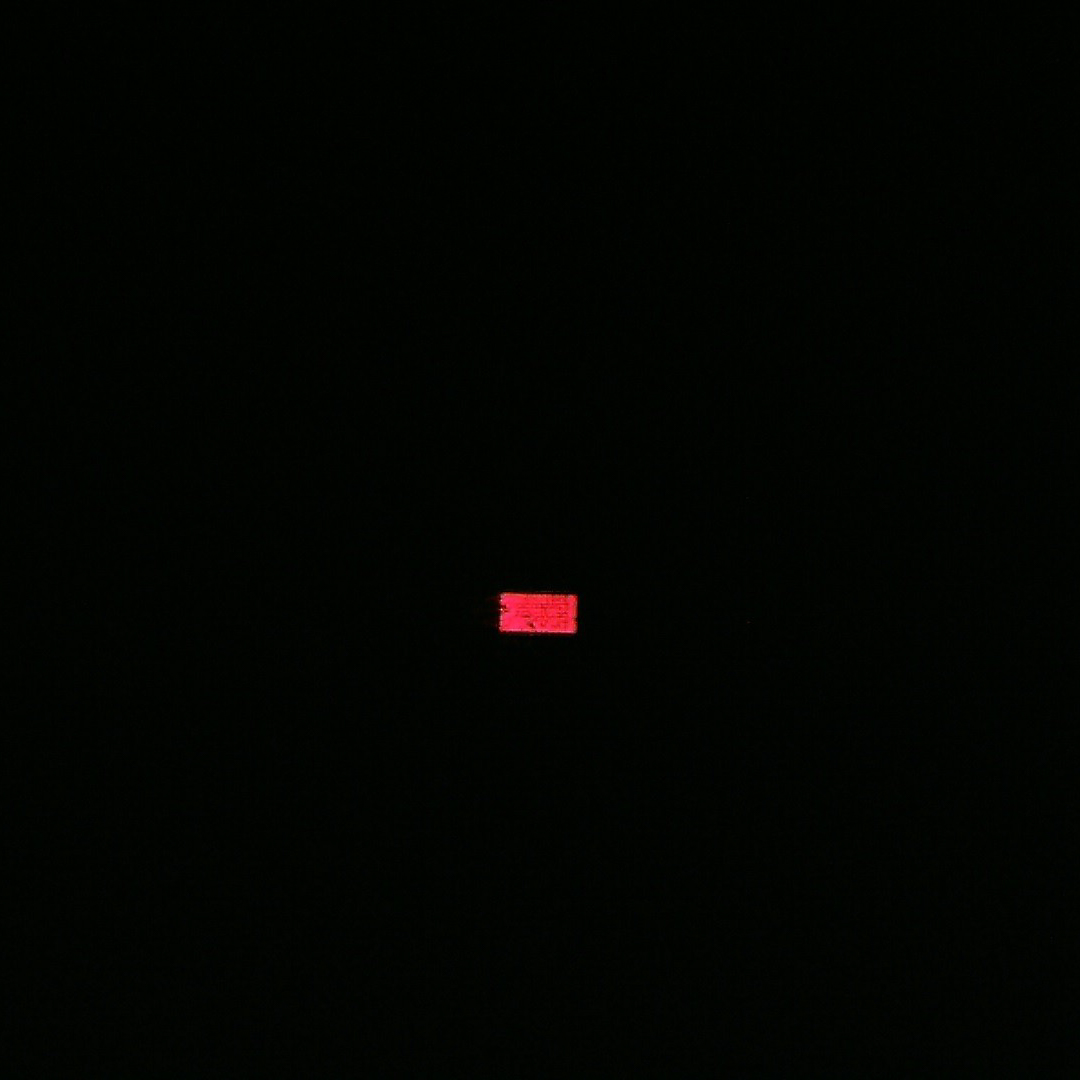
\includegraphics[width=\textwidth]{img-done/2-4.JPG}
        \captionsetup{font={normalsize,sf},justification=centering}
        \caption{矩形孔}
        \label{2-4}
    \end{subfigure}
    %%%%%%%%%%%%%%%%%%%%%%%%%%%%%
    \captionsetup{format=cont,justification=centering,subrefformat=parens}
    \caption{不同屏产生的频谱与像屏上图像}
\end{figure}
\clearpage
\begin{figure}[htbp]\ContinuedFloat
    \centering
    %%%%%%%%%%%%%%%%%%%%%%%%%%%%%
    \begin{subfigure}[htbp]{0.3\textwidth}
        \centering
        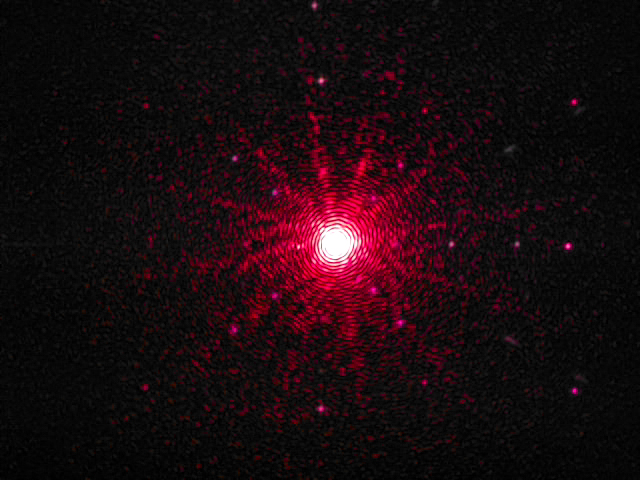
\includegraphics[width=\textwidth]{fre-done/2-5.JPG}
        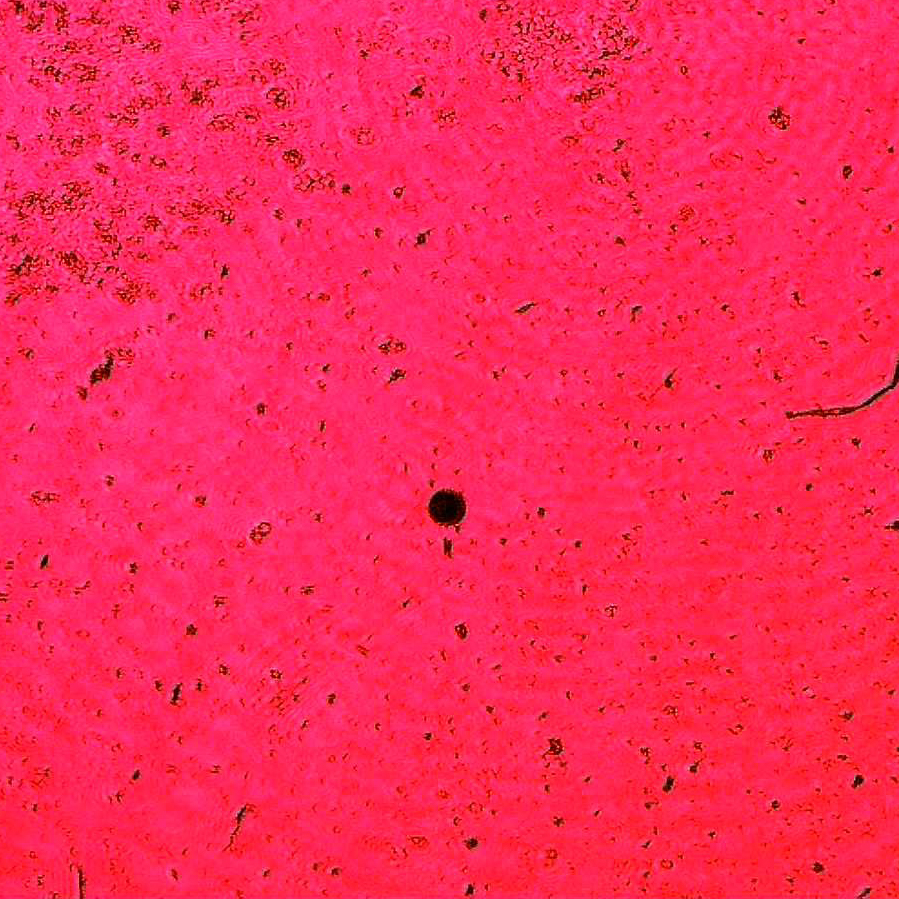
\includegraphics[width=\textwidth]{img-done/2-5.JPG}
        \captionsetup{font={normalsize,sf},justification=centering}
        \caption{单圆屏}
        \label{2-5}
    \end{subfigure}
    \begin{subfigure}[htbp]{0.3\textwidth}
        \centering
        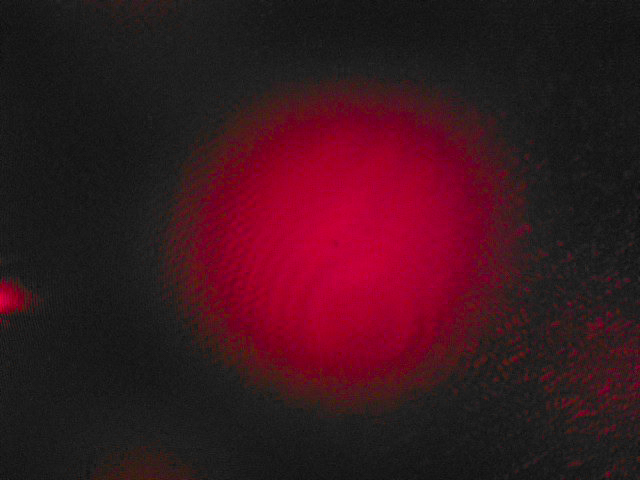
\includegraphics[width=\textwidth]{fre-done/2-6.JPG}
        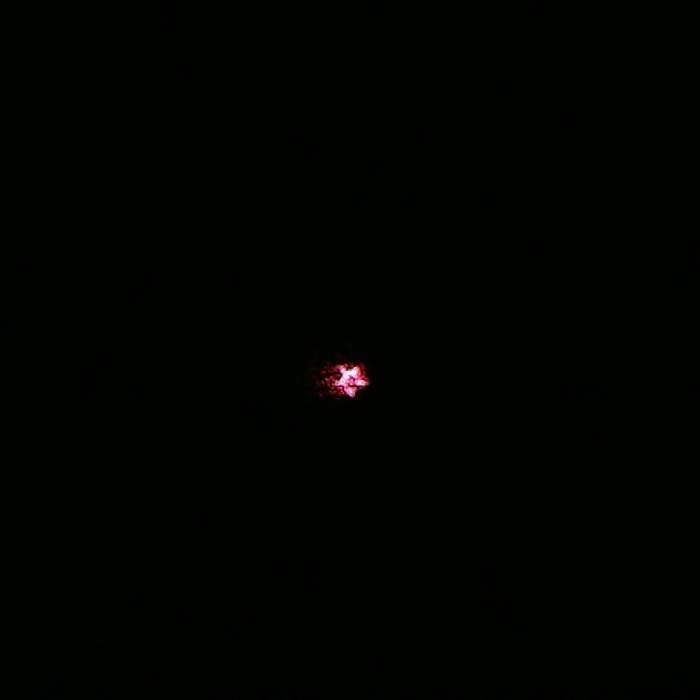
\includegraphics[width=\textwidth]{img-done/2-6.JPG}
        \captionsetup{font={normalsize,sf},justification=centering}
        \caption{五角星孔}
        \label{2-6}
    \end{subfigure}
    \begin{subfigure}[htbp]{0.3\textwidth}
        \centering
        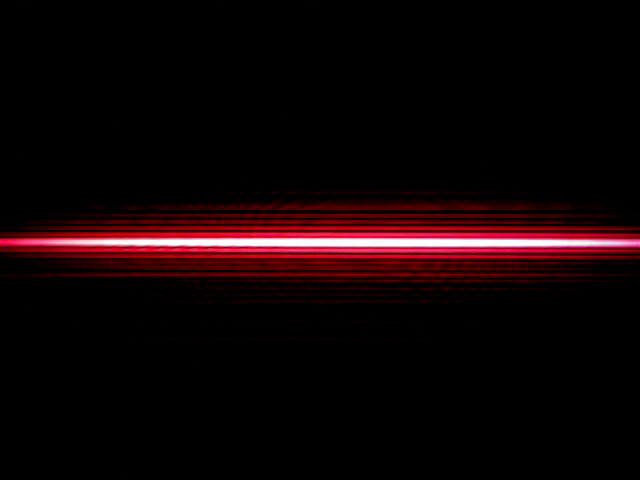
\includegraphics[width=\textwidth]{fre-done/2-7.JPG}
        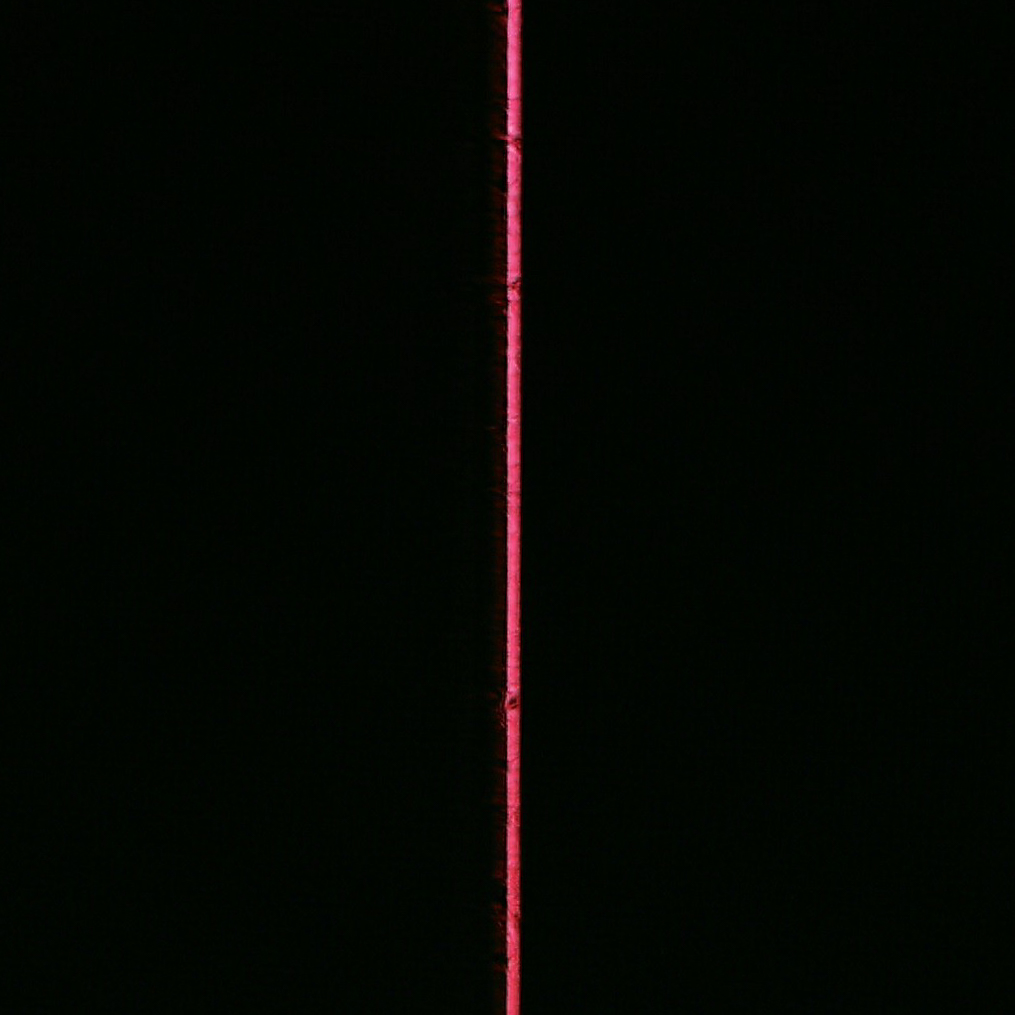
\includegraphics[width=\textwidth]{img-done/2-7.JPG}
        \captionsetup{font={normalsize,sf},justification=centering}
        \caption{单缝}
        \label{2-7}
    \end{subfigure}
    %%%%%%%%%%%%%%%%%%%%%%%%%%%%%
    \begin{subfigure}[htbp]{0.3\textwidth}
        \centering
        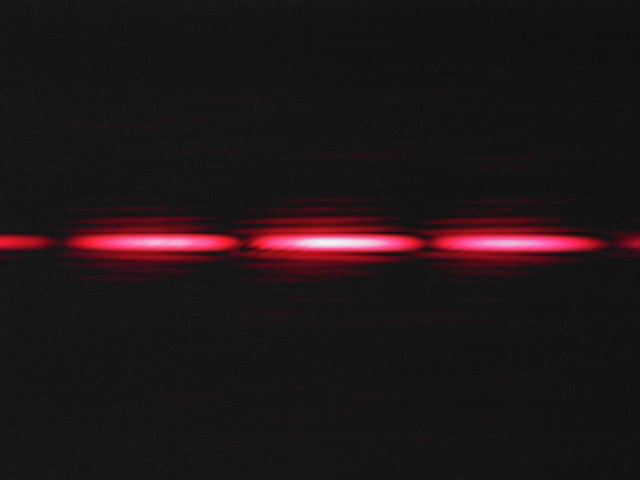
\includegraphics[width=\textwidth]{fre-done/2-8.JPG}
        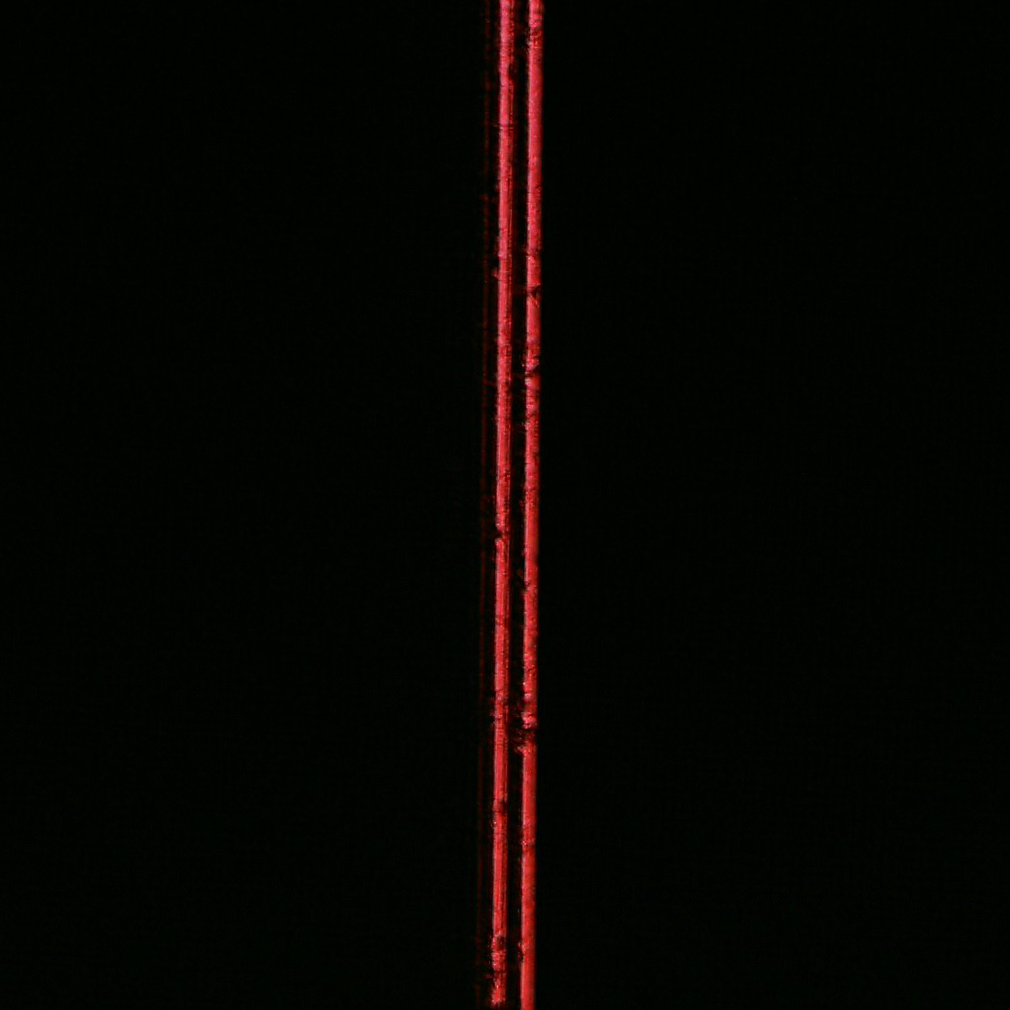
\includegraphics[width=\textwidth]{img-done/2-8.JPG}
        \captionsetup{font={normalsize,sf},justification=centering}
        \caption{双缝}
        \label{2-8}
    \end{subfigure}
    \begin{subfigure}[htbp]{0.3\textwidth}
        \centering
        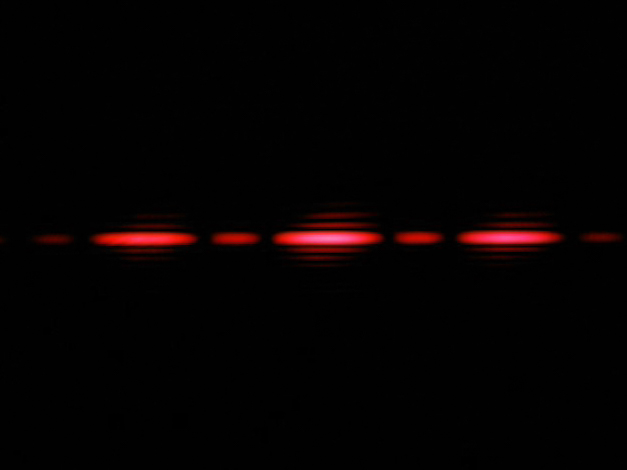
\includegraphics[width=\textwidth]{fre-done/3-1.JPG}
        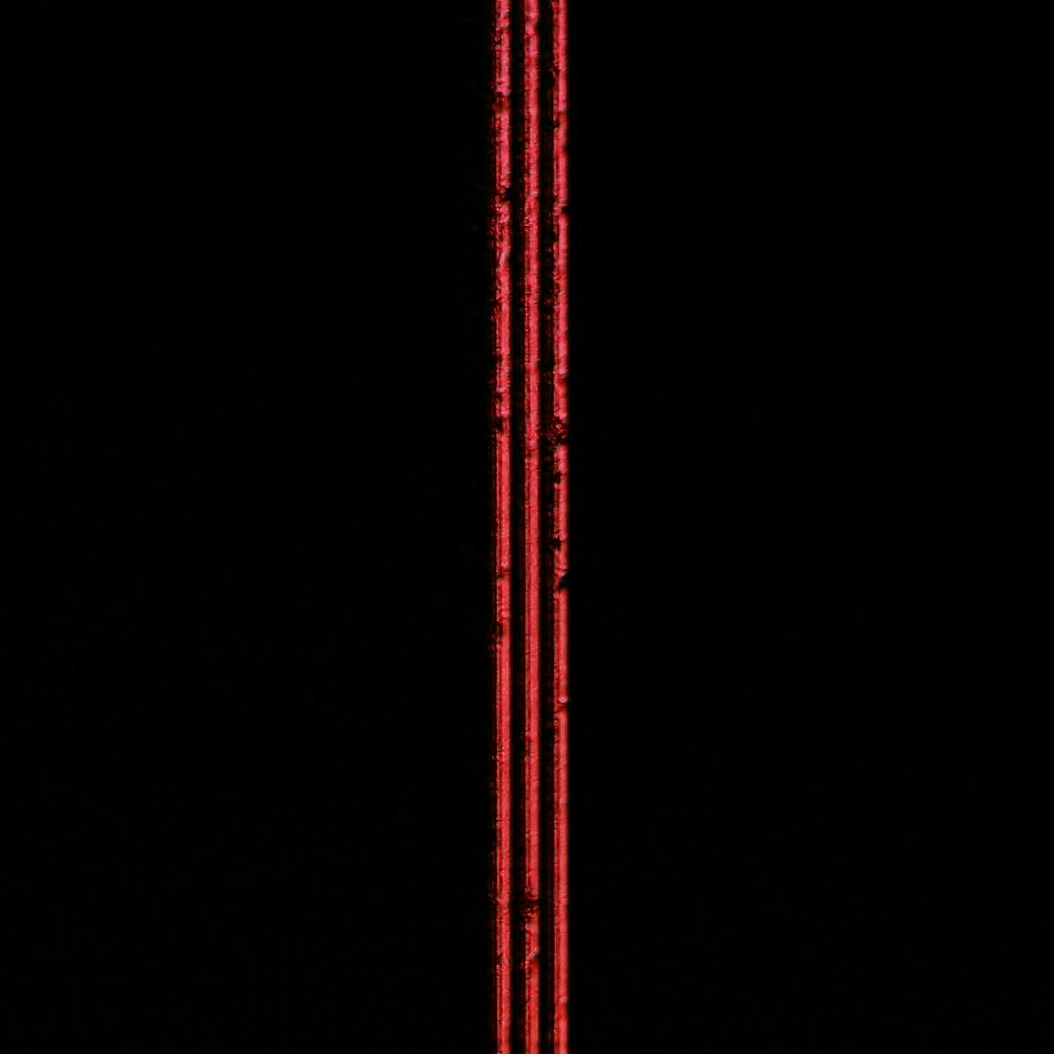
\includegraphics[width=\textwidth]{img-done/3-1.JPG}
        \captionsetup{font={normalsize,sf},justification=centering}
        \caption{三缝}
        \label{3-1}
    \end{subfigure}
    \begin{subfigure}[htbp]{0.3\textwidth}
        \centering
        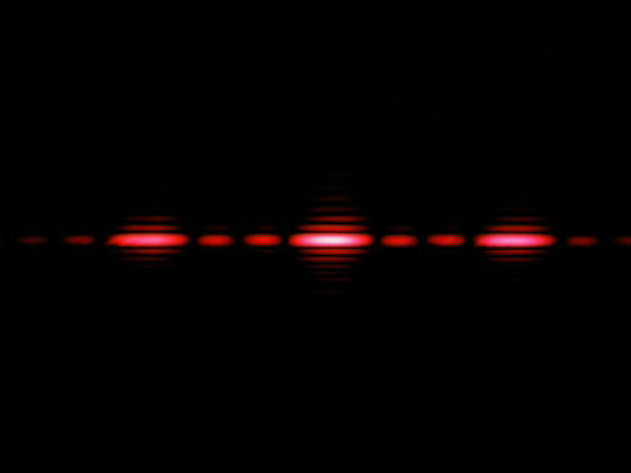
\includegraphics[width=\textwidth]{fre-done/3-2.JPG}
        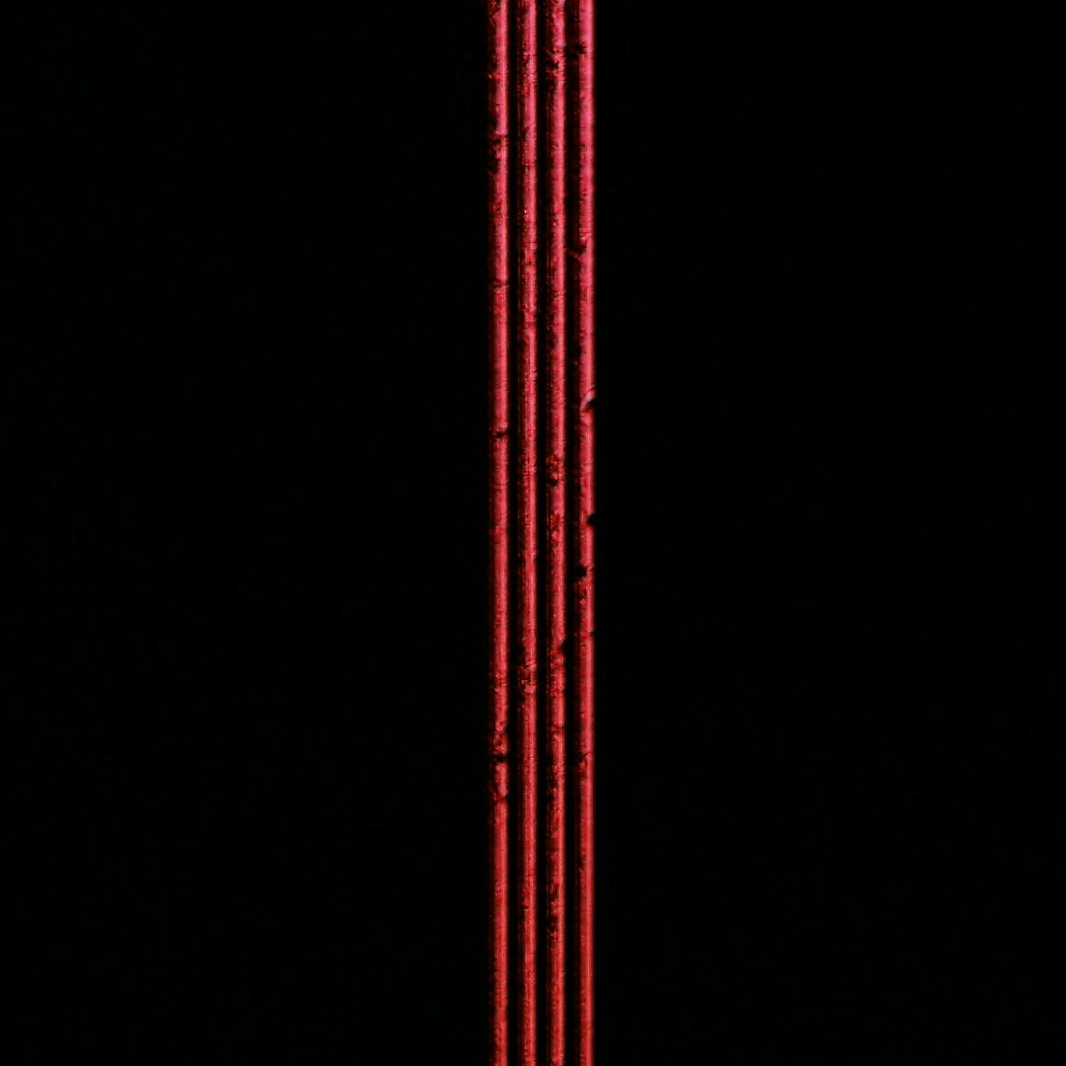
\includegraphics[width=\textwidth]{img-done/3-2.JPG}
        \captionsetup{font={normalsize,sf},justification=centering}
        \caption{四缝}
        \label{3-2}
    \end{subfigure}
    %%%%%%%%%%%%%%%%%%%%%%%%%%%%%
    \captionsetup{format=cont,justification=centering,subrefformat=parens}
    \caption{不同屏产生的频谱与像屏上图像}
\end{figure}
\clearpage
\begin{figure}[htbp]\ContinuedFloat
    \centering
    %%%%%%%%%%%%%%%%%%%%%%%%%%%%%
    \begin{subfigure}[htbp]{0.3\textwidth}
        \centering
        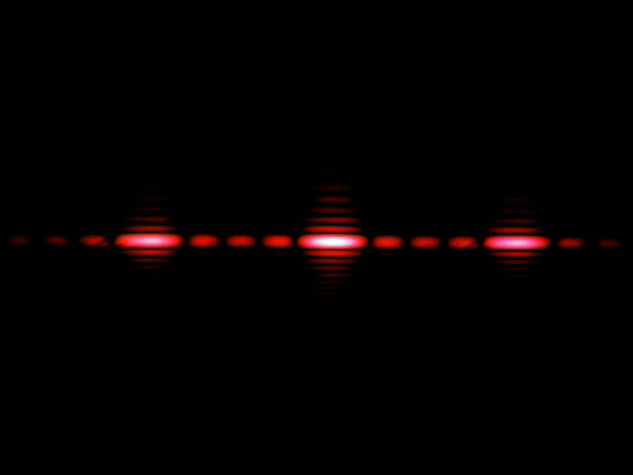
\includegraphics[width=\textwidth]{fre-done/3-3.JPG}
        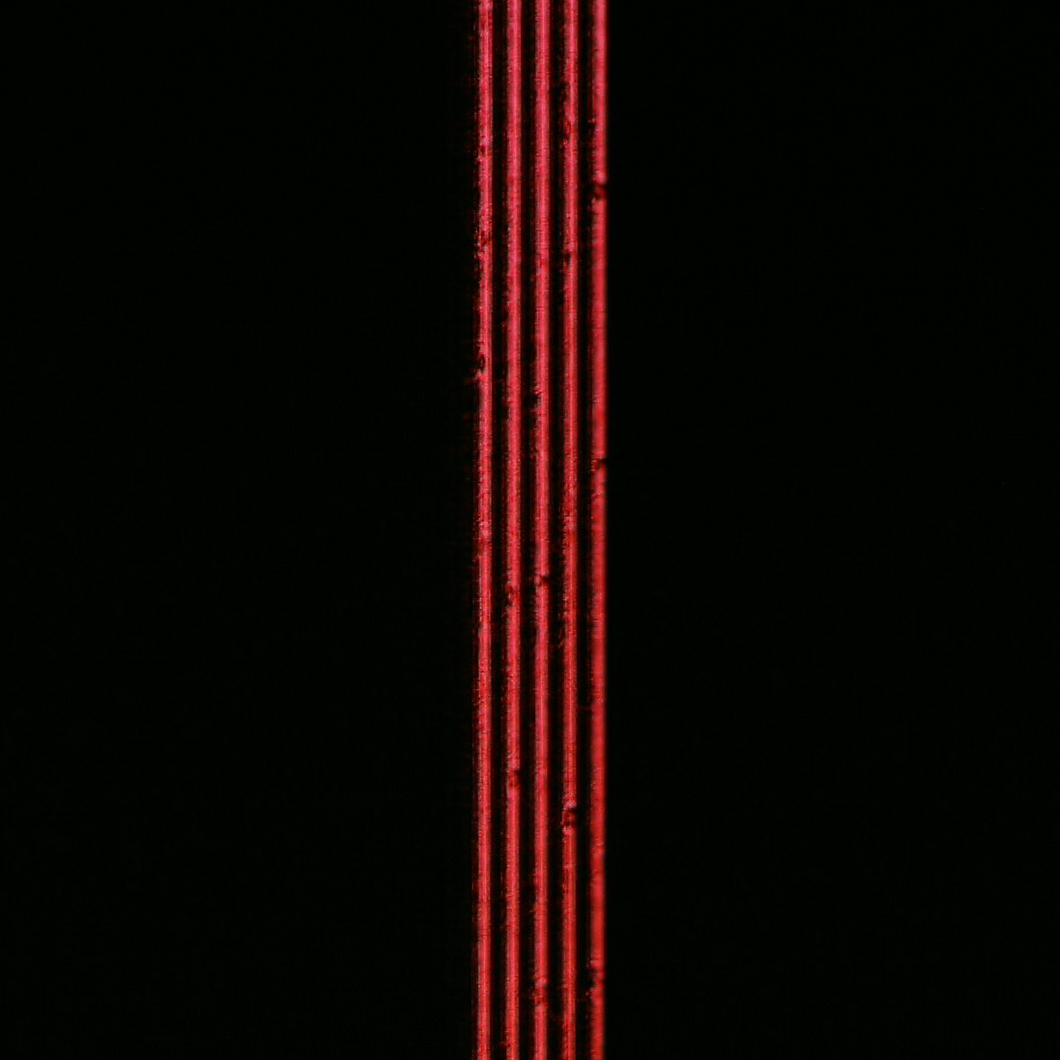
\includegraphics[width=\textwidth]{img-done/3-3.JPG}
        \captionsetup{font={normalsize,sf},justification=centering}
        \caption{五缝}
        \label{3-3}
    \end{subfigure}
    \begin{subfigure}[htbp]{0.3\textwidth}
        \centering
        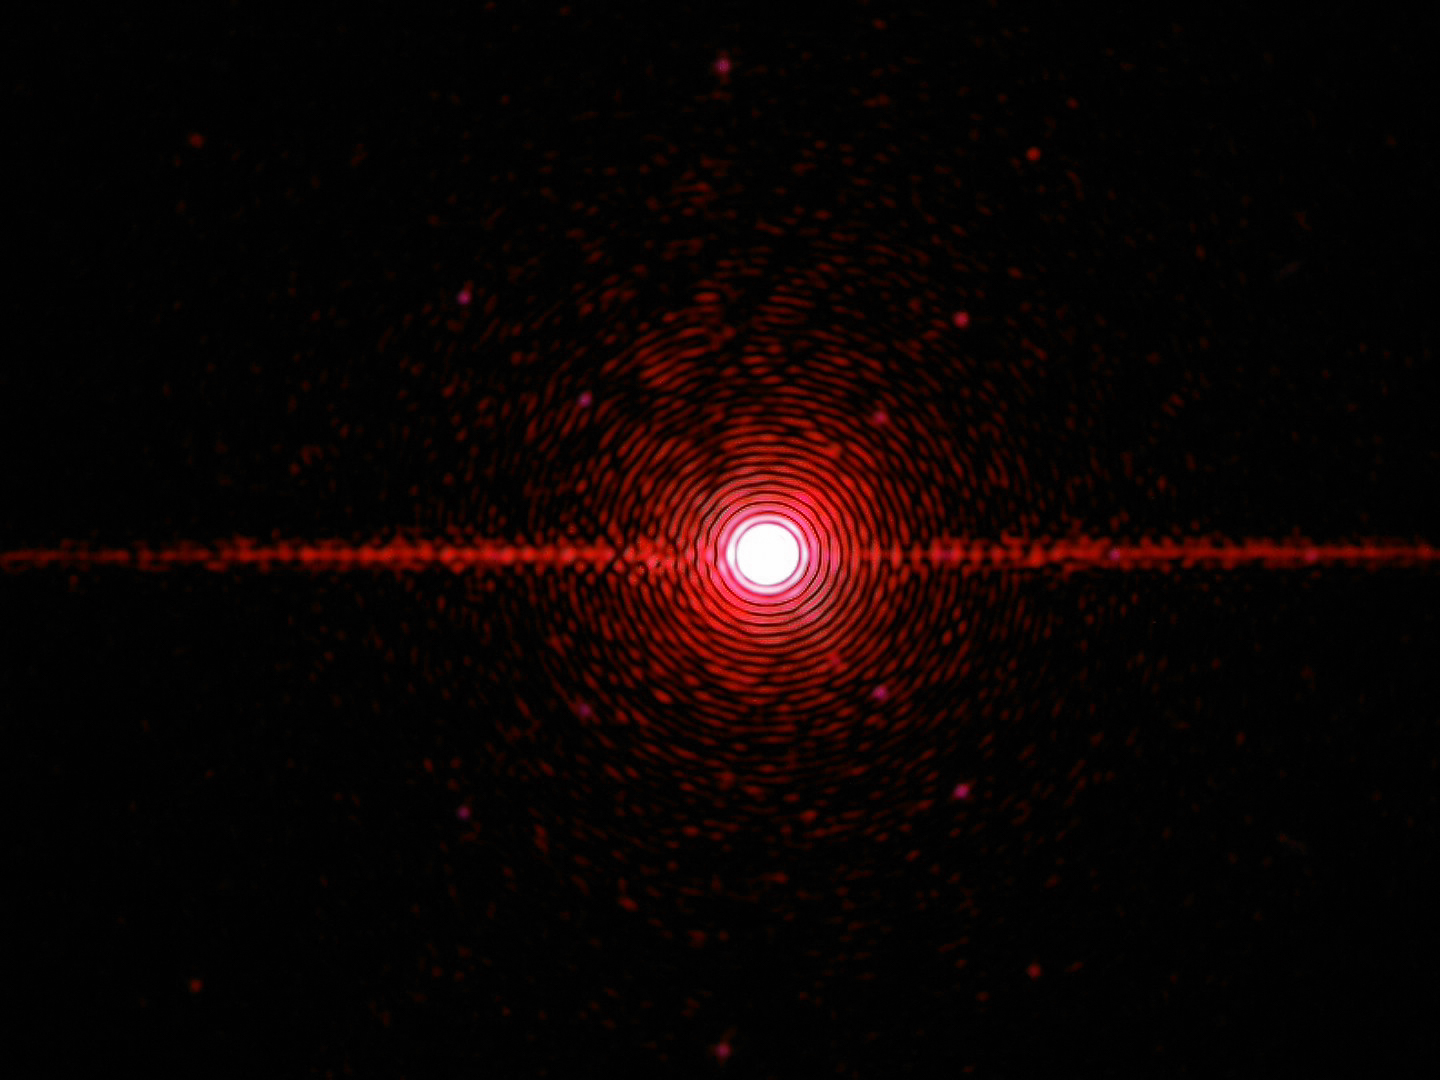
\includegraphics[width=\textwidth]{fre-done/3-4.JPG}
        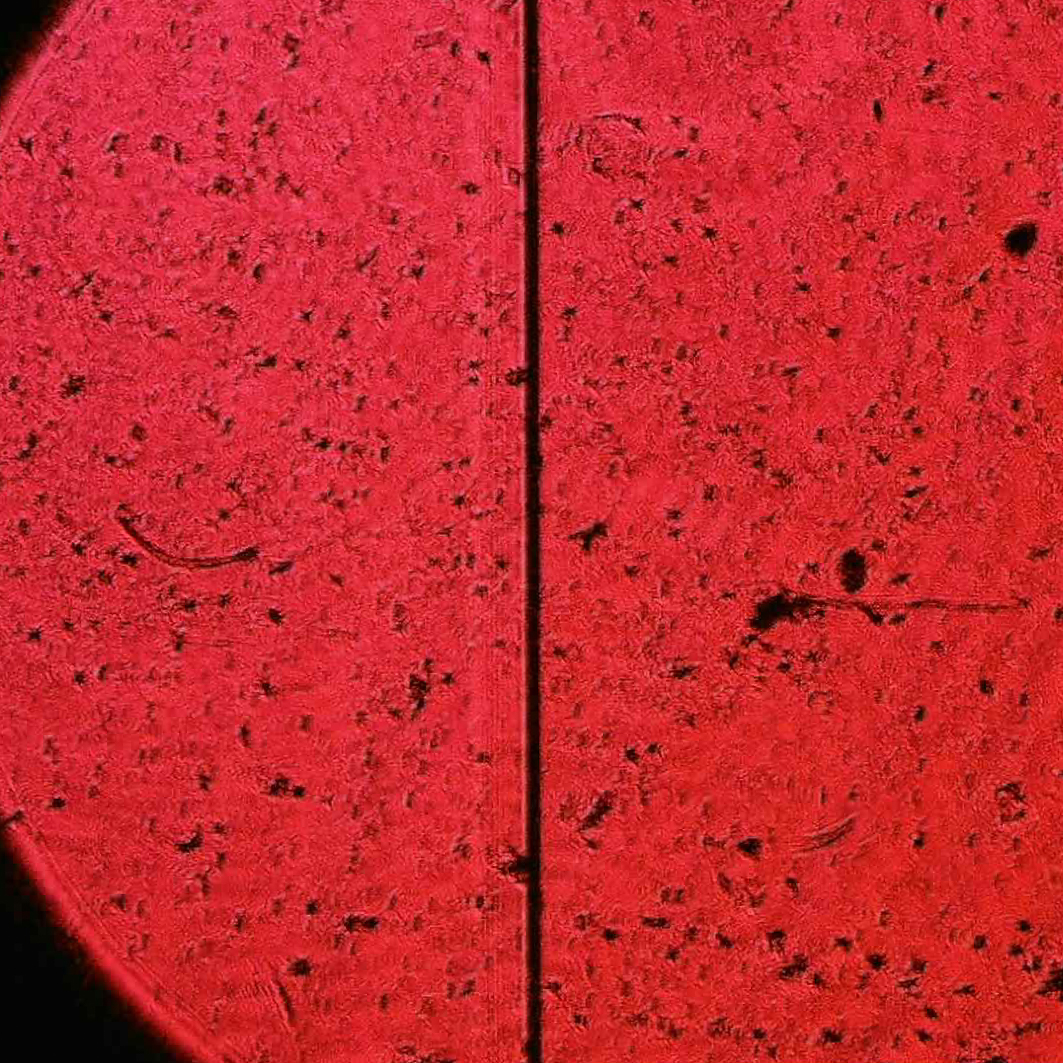
\includegraphics[width=\textwidth]{img-done/3-4.JPG}
        \captionsetup{font={normalsize,sf},justification=centering}
        \caption{单丝}
        \label{3-4}
    \end{subfigure}
    \begin{subfigure}[htbp]{0.3\textwidth}
        \centering
        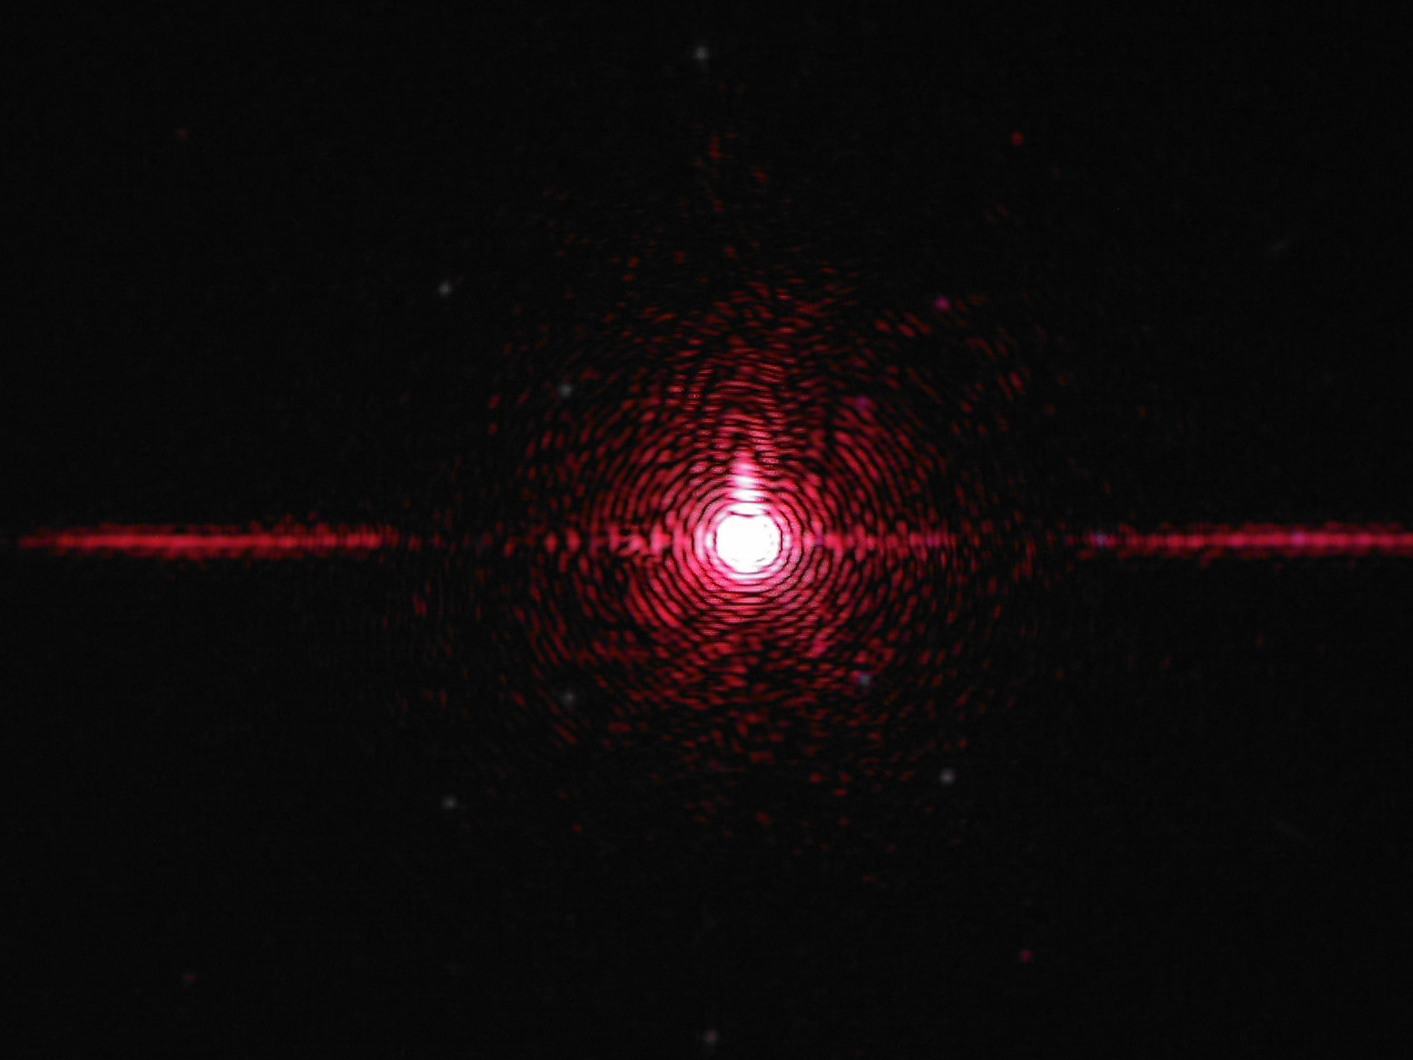
\includegraphics[width=\textwidth]{fre-done/3-5.JPG}
        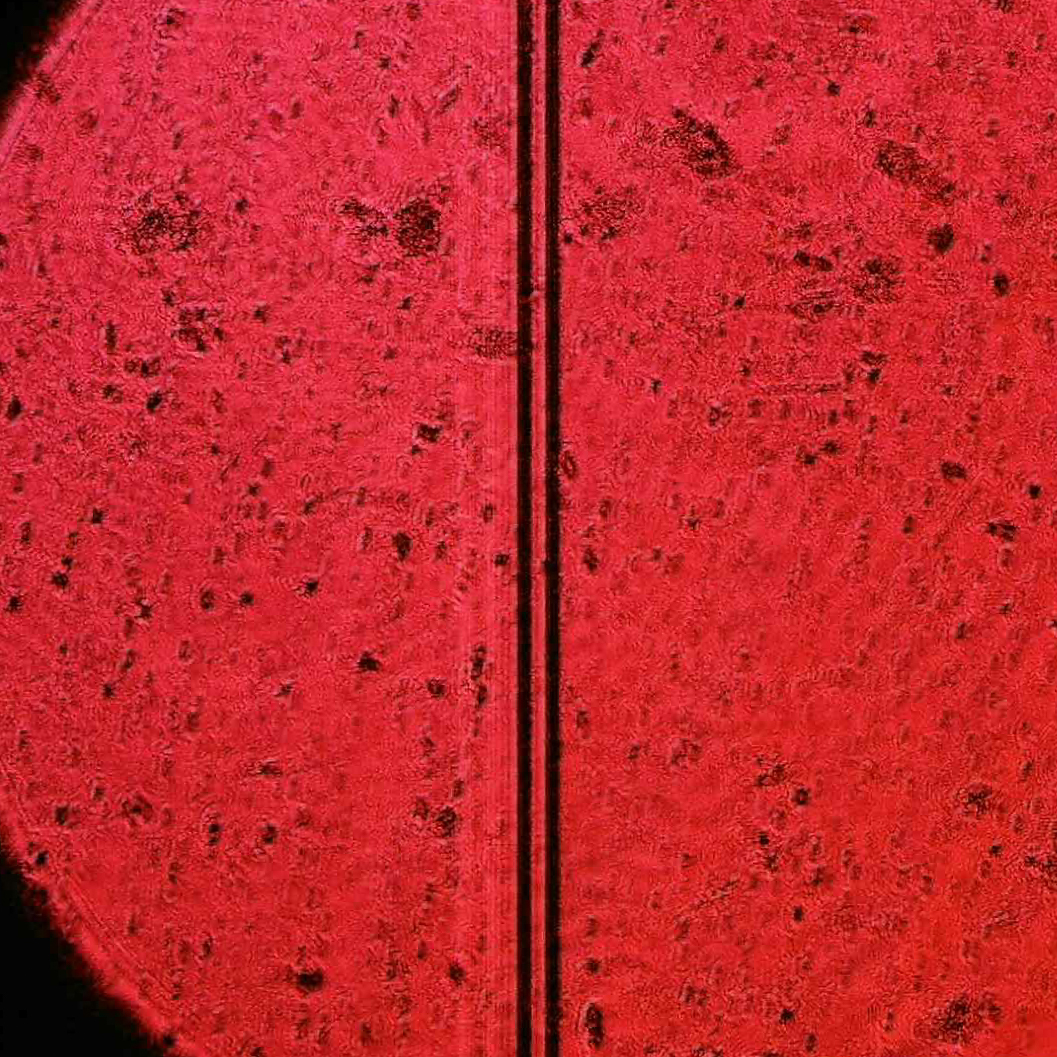
\includegraphics[width=\textwidth]{img-done/3-5.JPG}
        \captionsetup{font={normalsize,sf},justification=centering}
        \caption{双丝}
        \label{3-5}
    \end{subfigure}
    %%%%%%%%%%%%%%%%%%%%%%%%%%%%%
    \begin{subfigure}[htbp]{0.3\textwidth}
        \centering
        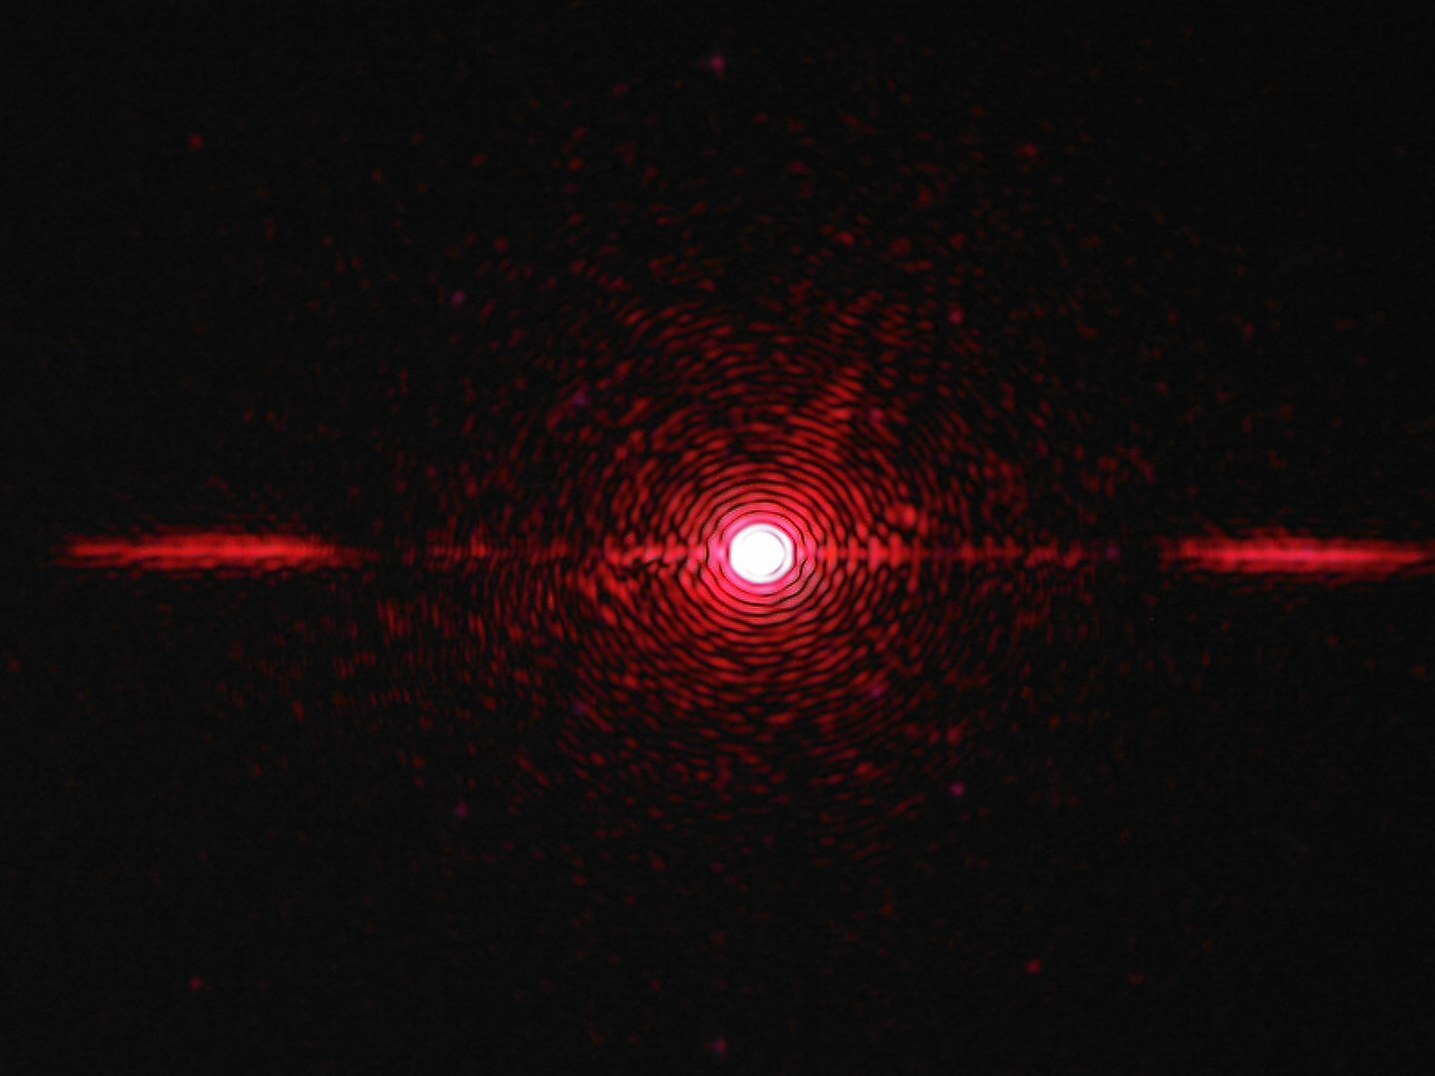
\includegraphics[width=\textwidth]{fre-done/3-6.JPG}
        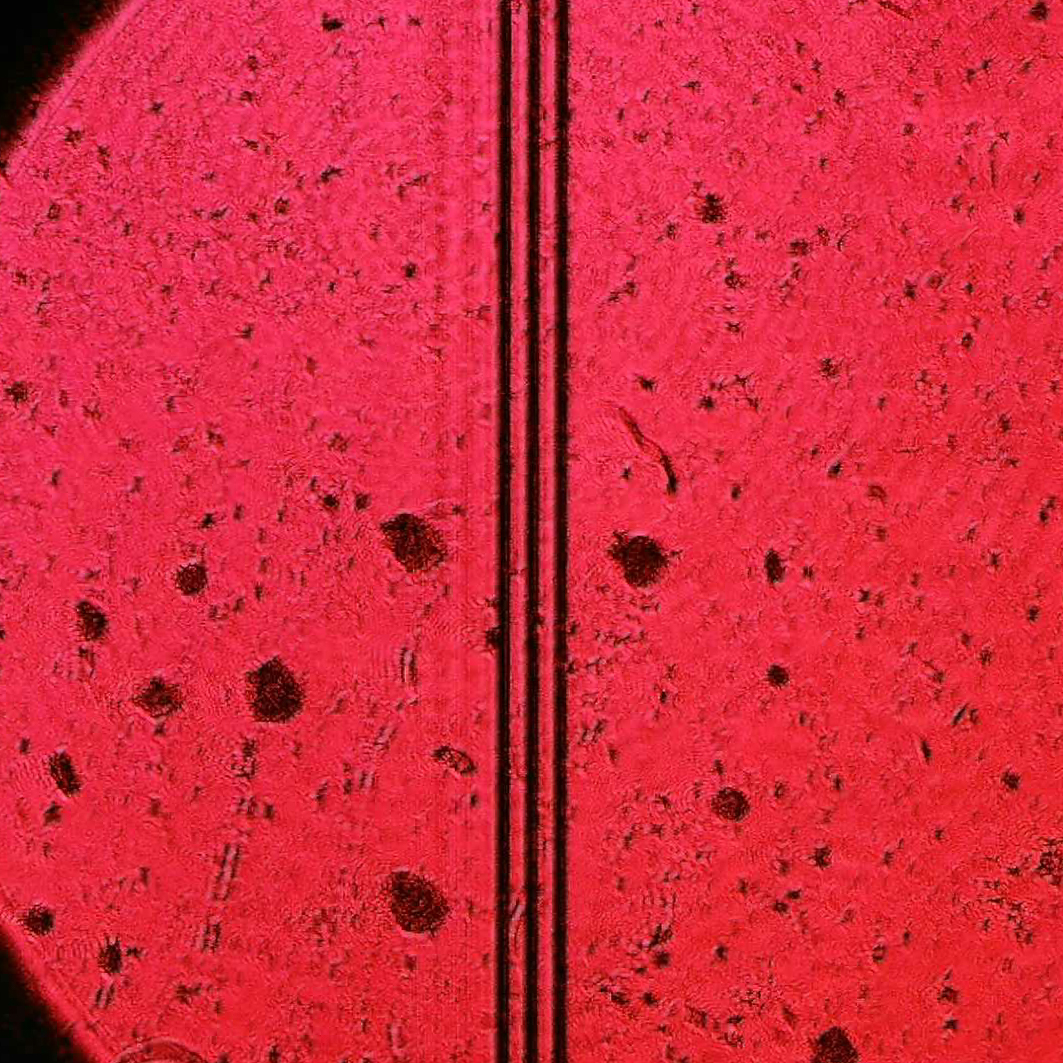
\includegraphics[width=\textwidth]{img-done/3-6.JPG}
        \captionsetup{font={normalsize,sf},justification=centering}
        \caption{三丝}
        \label{3-6}
    \end{subfigure}
    \begin{subfigure}[htbp]{0.3\textwidth}
        \centering
        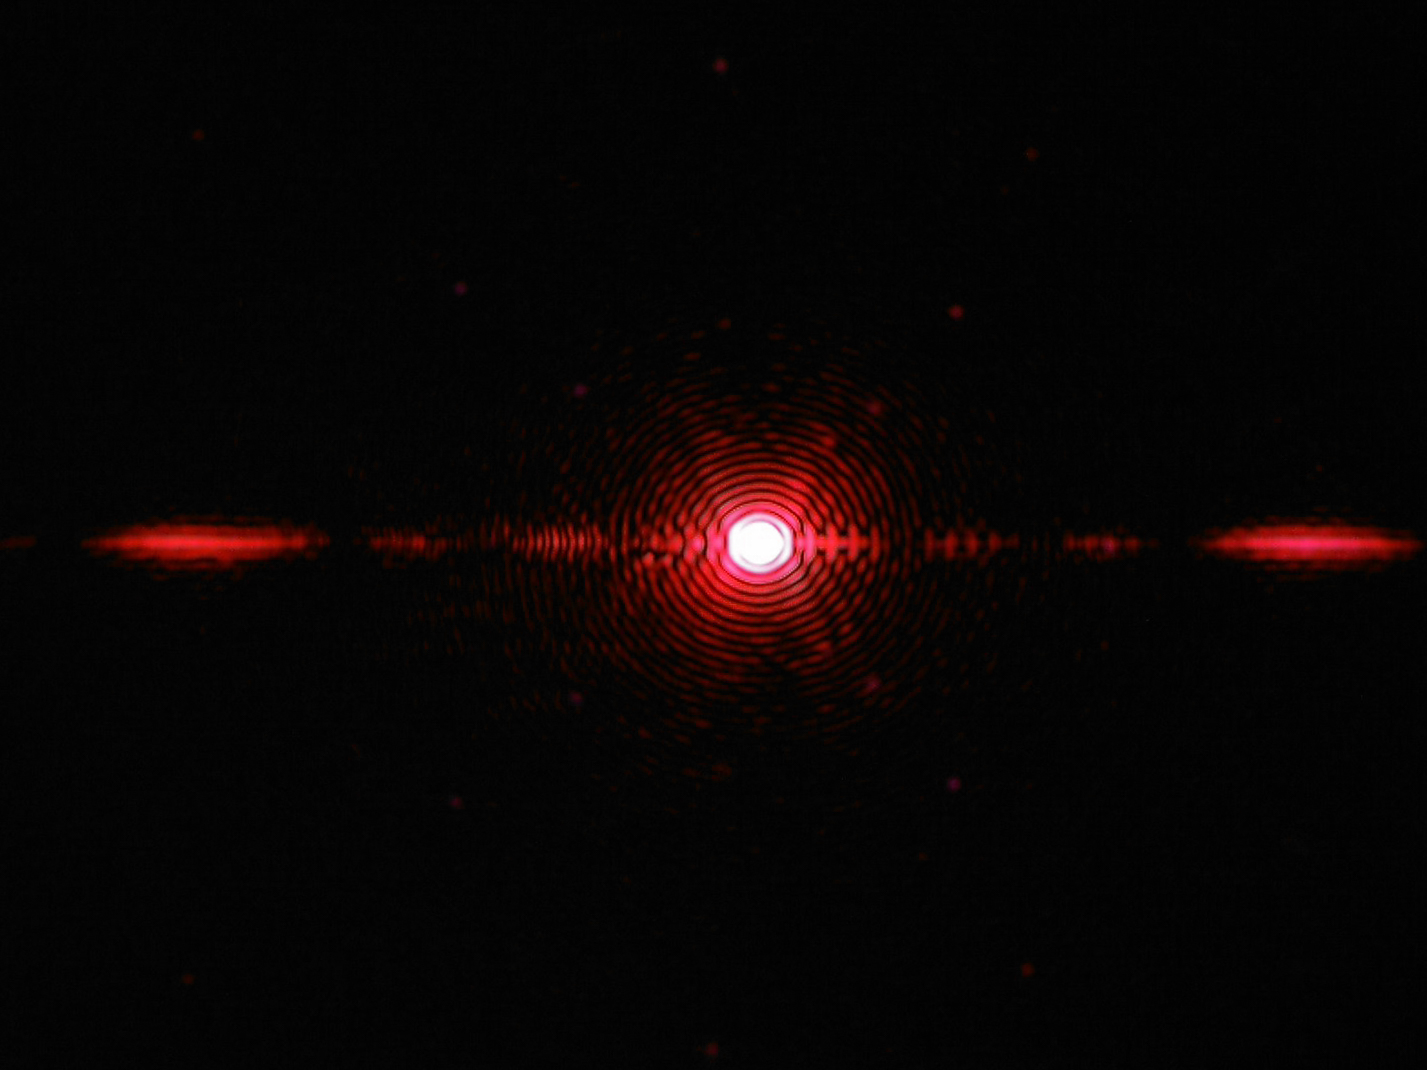
\includegraphics[width=\textwidth]{fre-done/3-7.JPG}
        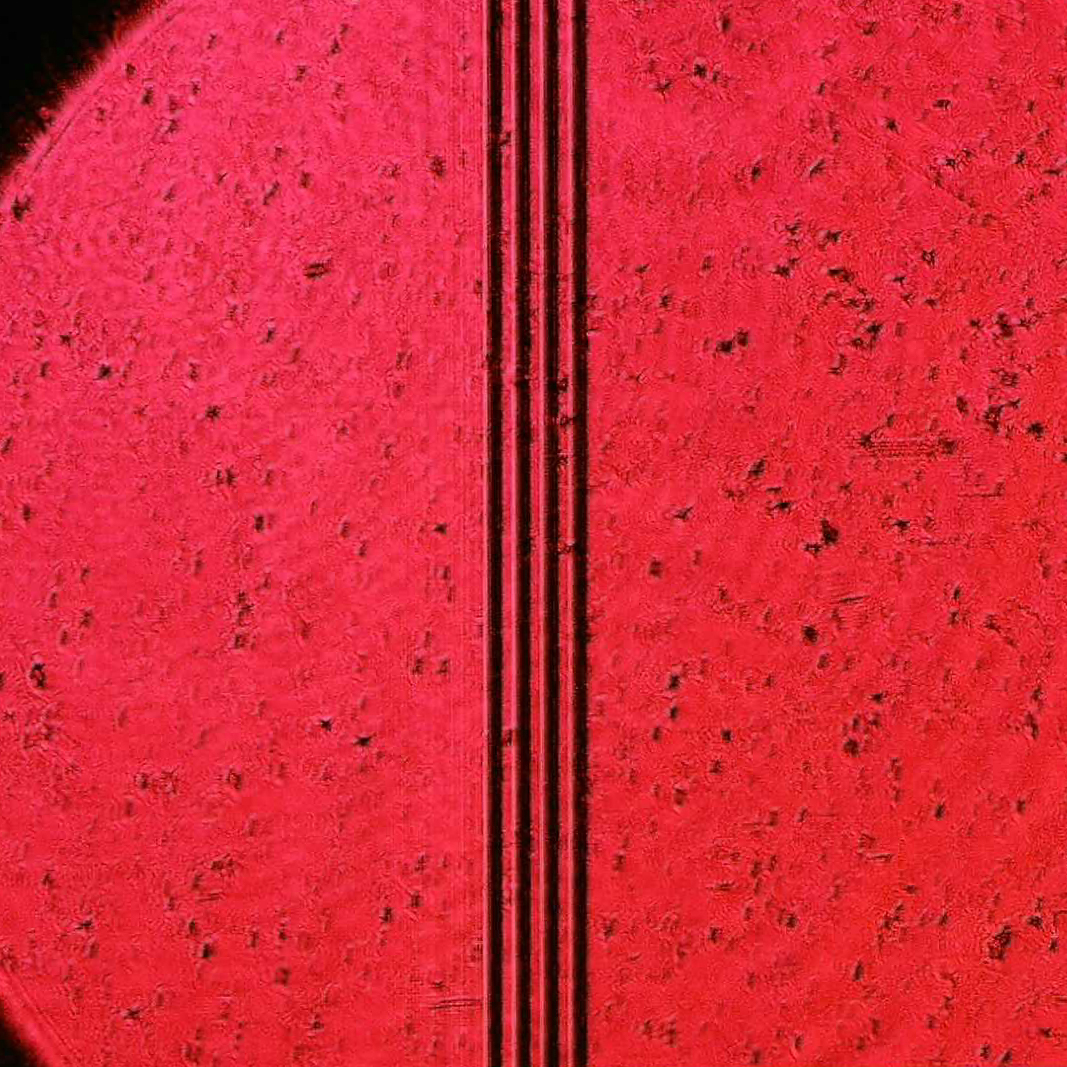
\includegraphics[width=\textwidth]{img-done/3-7.JPG}
        \captionsetup{font={normalsize,sf},justification=centering}
        \caption{四丝}
        \label{3-7}
    \end{subfigure}
    \begin{subfigure}[htbp]{0.3\textwidth}
        \centering
        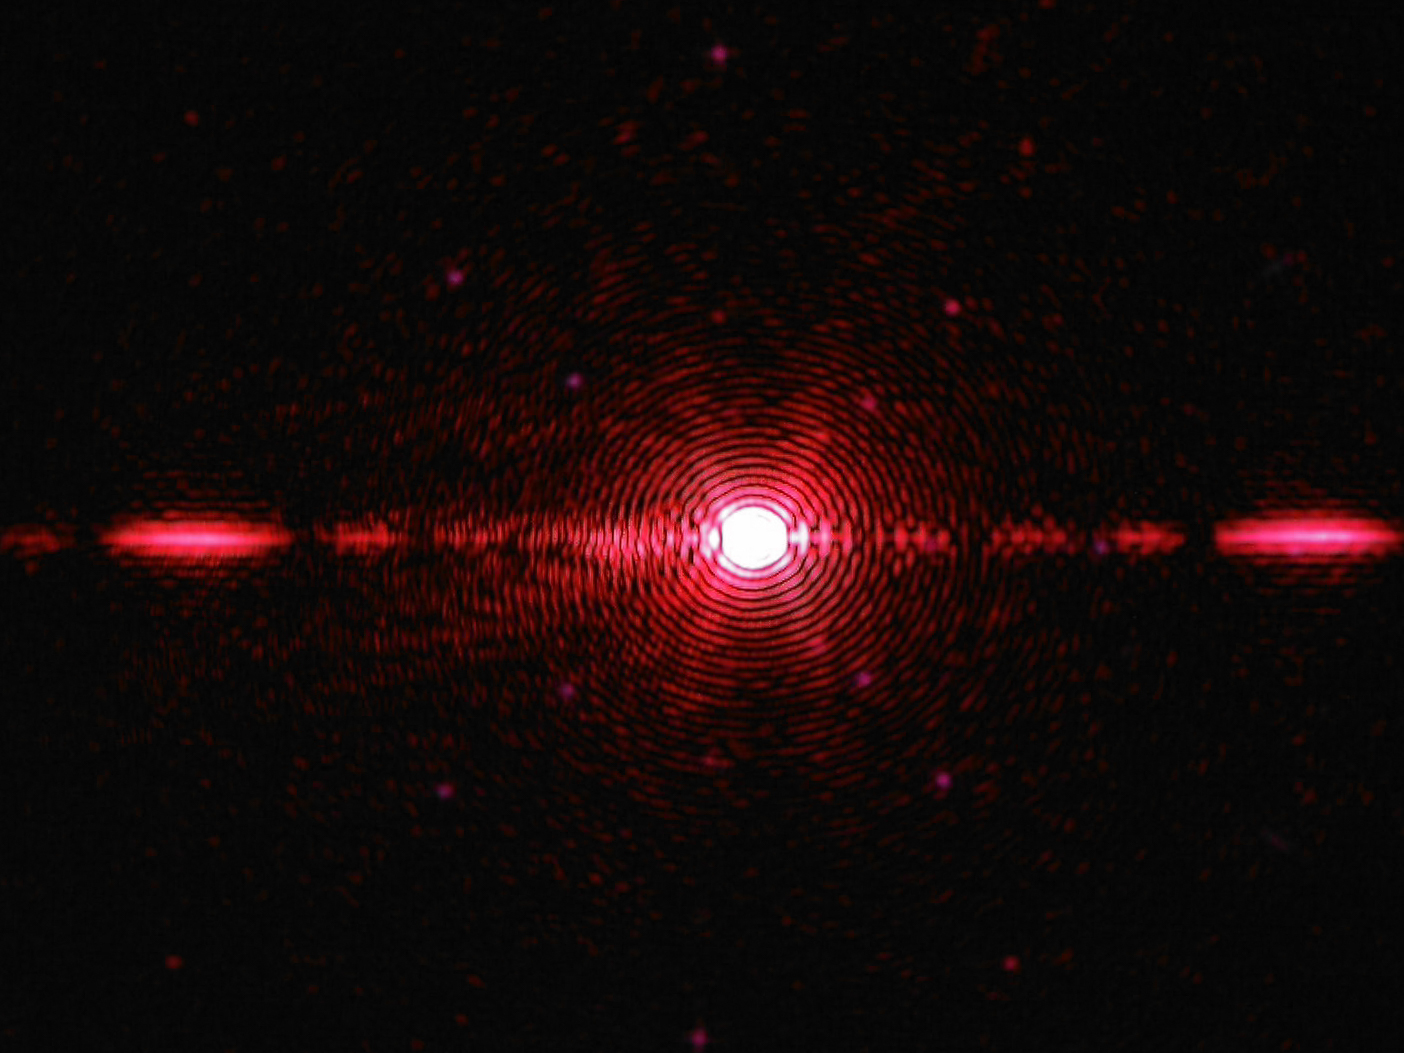
\includegraphics[width=\textwidth]{fre-done/3-8.JPG}
        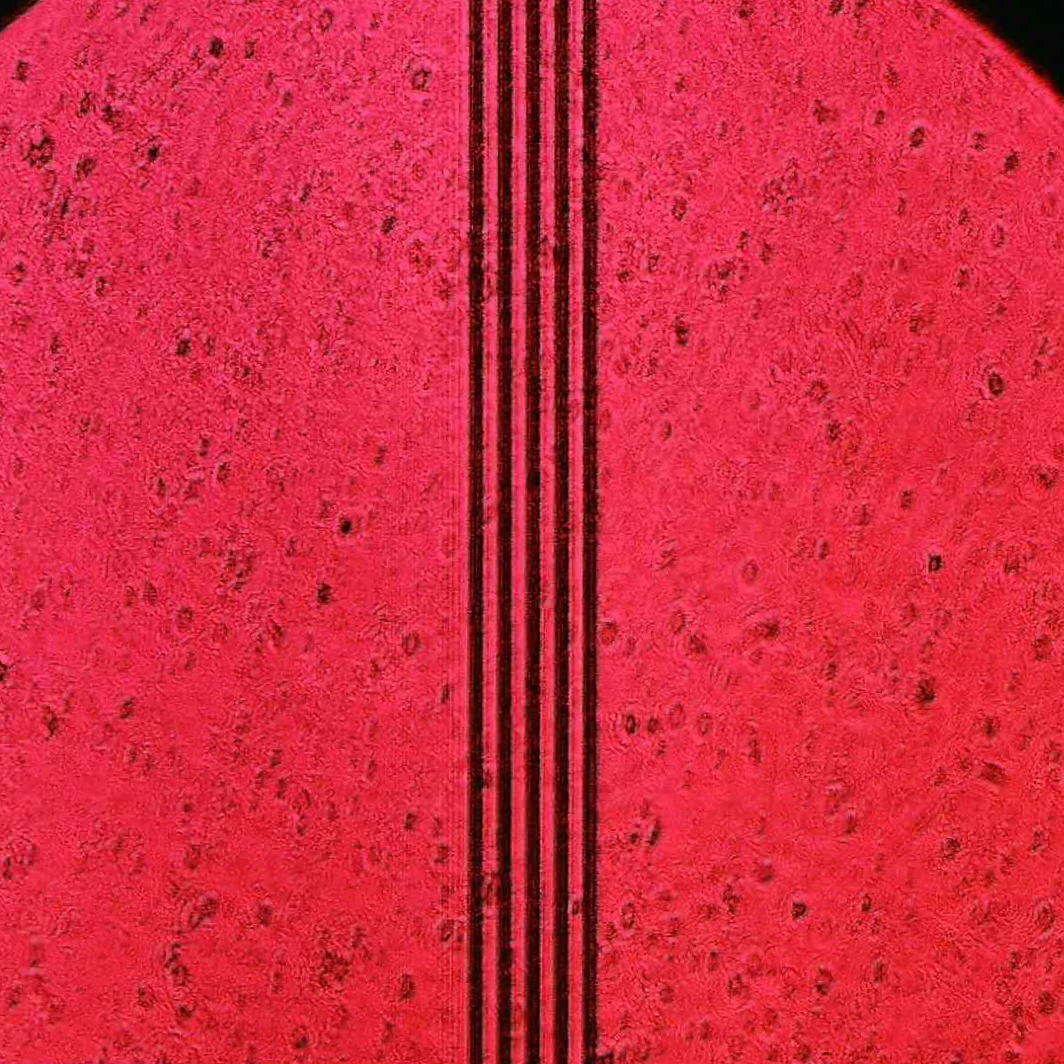
\includegraphics[width=\textwidth]{img-done/3-8.JPG}
        \captionsetup{font={normalsize,sf},justification=centering}
        \caption{五丝}
        \label{3-8}
    \end{subfigure}
    %%%%%%%%%%%%%%%%%%%%%%%%%%%%%
    \captionsetup{format=cont,justification=centering,subrefformat=parens}
    \caption{不同屏产生的频谱与像屏上图像}
\end{figure}
\clearpage

\hspace{2em}对于(\subref{1-3})方孔方阵:两个相互垂直的两个方向都可类比为多缝,而正方形口口孔则决定其主极大和次极大位置,参考(\subref{1-1})方孔屏:可以见到其在对角线方向上的条纹是比较多的。(\subref{1-4})方孔密排:与(\subref{1-3})相比,其空间周期有所变化,其特征方向改变,具体可以使用相移-位移定理来作推算,但其主要构成单元也是多个鏠,因此也会出现一个个暗小方格的情况。\par
\hspace{2em}对于(\subref{1-7})圆孔方阵:对比(\subref{1-3}),由于圆孔子结构的调制,其对角线方向上的条纹相对较小。(\subref{1-8})圆孔密排:由于圆孔小结构对离中心亮纹的半径$R$一样的地方进行相同的调制,因此也可以看清图中四个角落处的条变,而方孔的田个角落为极小值的位置,没有明显条纹。\par

%%%%%%%%%%%%%%%%%%%%%%%%%%%%%%%%%%%%%%%%%%%%%%%%%%%%%%%%%%%%%%%%%%%

\subsection{光栅的衍射}

%%%%%%%%%%%%%%%%%%%%%%%%%%%%%%%%%%%%%%%%%%%%%%%

\subsubsection{测量一维光栅衍射的各空间频率并求光栅的基频}
\hspace{2em}透镜焦距为$f=25cm$,激光器波长$\lambda=\SI{632.8}{\nm}$。\par
\hspace{2em}利用一维光栅空间频率公式:\par
$$f_x=\frac{\Delta x}{\lambda f}$$
\hspace{2em} 对上述光路进行测量,得到下表: \par
\begin{table}[htbp]
    \centering
    \captionsetup{justification=centering,margin=2cm}
    \caption{衍射级次以及相应的位置及空间频率表\label{table:1}}
    \setlength{\tabcolsep}{10mm}
    \renewcommand{\arraystretch}{1.1}
    {\begin{tabular}{ccc}
            \toprule
            衍射级次 & 位置$\Delta x/\SI{}{\mm}$ & 空间频率$f_x/\SI{}{\per\mm}$ \\
            \midrule
            1        & 1.9                       & 12.0                         \\
            2        & 3.8                       & 24.0                         \\
            3        & 5.7                       & 36.0                         \\
            4        & 7.6                       & 48.0                         \\
            5        & 9.5                       & 60.0                         \\
            6        & 11.4                      & 72.0                         \\
            \bottomrule
        \end{tabular}}
\end{table}\par
\hspace{2em} 进行拟合后可以得到光栅的空间频率: \par
$$\bar{f_x}=\SI{12.0}{\per\mm}$$

%%%%%%%%%%%%%%%%%%%%%%%%%%%%%%%%%%%%%%%%%%%%%%%

\subsubsection{在频谱面放上可调狭缝及其他附加光栏进行空间滤波,记录像面特点及条纹间距}
\hspace{2em} 由傅里叶三角级数形式: \par
$$T_n(x)=\frac{a_0}{2}+ \sum^\infty_{k=1}a_k\cos{k x}+b_k\sin{k x}$$
\clearpage
\hspace{2em} 对不同的空间滤波条件进行讨论: \par
\begin{table}[htbp]
    \centering
    \captionsetup{justification=centering,margin=2cm}
    \caption{不同空间滤波条件讨论\label{table:2}}
    \setlength{\tabcolsep}{3mm}
    \renewcommand{\arraystretch}{1.4}
    {\begin{tabular}{m{1cm}<{\centering}m{2.3cm}<{\centering}m{4.5cm}<{\centering}m{5cm}<{\centering}}
            \toprule
            条件 & 通过的衍射点  & \tableCenter{图像情况}                                                     & \tableCenter{简要解释}                                                                                                                    \\\midrule
            A    & 全部          & 等间距的亮条纹和暗条纹。                                          & 利用傅里叶三角级数形式,一维光栅的像在屏上为周期性的方波。                                                                       \\
            B    & 0级           & 用内眼看屏时,基本看不出亮条纹和暗条纹。                          & 由于丢失了全部周期性变化的交流信息,因此像面上呈现一片均匀强度的光。                                                             \\
            C    & 0,$\pm 1$级   & 和A间距一样的亮条纹和暗条纹。                                     & 这与A的图像差别不大,但傅里叶三角级数形式会发现只剩下$\pm 1$级频率的三角函数,因此在屏上为一余弦函数。                           \\
            D    & 除$\pm 1$级外 & 频率为A两倍的的亮条纹和暗条纹                                     & 由于$\pm 1$级频率的三角函数(占主要地位)没有了,使$\pm 2$级频率的三角函数代替,因此条纹间距变为原来的二分之一。                   \\
            E    & 除0级外       & 和A间距一样的亮条纹和暗条纹,亮纹之间的暗纹对比之前的亮纹稍亮一些 & 复振幅分布没有了直流成份,但由于透镜相当于一个低通滤波器,使得一部分高频信息滤掉使原本不透光部位也变亮了(这种现象称为衬比度反转) \\
            \bottomrule
        \end{tabular}}
\end{table}\par
\hspace{2em} 其具体物理原因如下图所示,假定光栅常数与缝寛满足$\frac{a}{d}=\frac{2}{3}$,并且由于透镜的关系,最多只能容许$100f_x$的频率通过,\par
\begin{figure}[H]
    \centering
    %%%%%%%%%%%%%%%%%%%%%%%%%%%%%
    \begin{subfigure}[t]{0.45\textwidth}
        \centering
        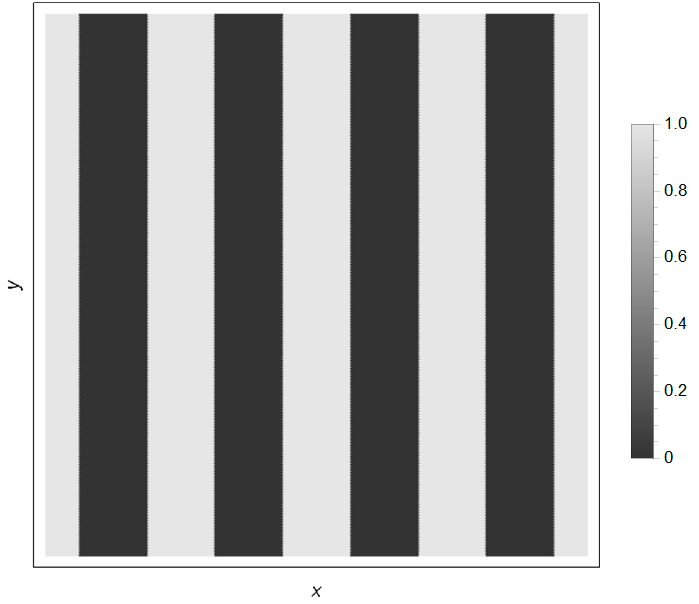
\includegraphics[height=\textheight/4]{simu/lightgate.png}
        \captionsetup{font={normalsize,sf},justification=centering}
        \caption{一维光栅的屏函数}
        \label{fig3-1}
    \end{subfigure}
    %%%%%%%%%%%%%%%%%%%%%%%%%%%%%
    \begin{subfigure}[t]{0.45\textwidth}
        \centering
        \includegraphics[height=\textheight/4]{simu/frelg.png}
        \captionsetup{font={normalsize,sf},justification=centering}
        \caption{频谱示意图}
        \label{fig3-2}
    \end{subfigure}
    %%%%%%%%%%%%%%%%%%%%%%%%%%%%%
    \captionsetup{justification=centering,subrefformat=parens,margin=2cm}
    \caption{一维光栅衍射空间滤波示意图;\subref{fig3-2}由\subref{fig3-1}经过一次傅立叶变换$\mathcal{F}(x)$得到,然后再加入不同的狭缝来控制不同频率的通过。}
\end{figure}
\begin{figure}[H]\ContinuedFloat
    \centering
    %%%%%%%%%%%%%%%%%%%%%%%%%%%%%
    \begin{subfigure}[t]{0.4\textwidth}
        \centering
        \includegraphics[width=\textwidth]{simu/A.png}
        \captionsetup{font={normalsize,sf},justification=centering}
        \caption{全部通过}
        \label{fig3-3-1}
    \end{subfigure}
    %%%%%%%%%%%%%%%%%%%%%%%%%%%%%
    \begin{subfigure}[t]{0.4\textwidth}
        \centering
        \includegraphics[width=\textwidth]{simu/Aimg.png}
        \captionsetup{font={normalsize,sf},justification=centering}
        \caption{}
        \label{fig3-3-2}
    \end{subfigure}
    %%%%%%%%%%%%%%%%%%%%%%%%%%%%%
    \begin{subfigure}[t]{0.4\textwidth}
        \centering
        \includegraphics[width=\textwidth]{simu/B.png}
        \captionsetup{font={normalsize,sf},justification=centering}
        \caption{$0$级通过}
        \label{fig3-3-3}
    \end{subfigure}
    %%%%%%%%%%%%%%%%%%%%%%%%%%%%%
    \begin{subfigure}[t]{0.4\textwidth}
        \centering
        \includegraphics[width=\textwidth]{simu/Bimg.png}
        \captionsetup{font={normalsize,sf},justification=centering}
        \caption{}
        \label{fig3-3-4}
    \end{subfigure}
    %%%%%%%%%%%%%%%%%%%%%%%%%%%%%
    \begin{subfigure}[t]{0.4\textwidth}
        \centering
        \includegraphics[width=\textwidth]{simu/C.png}
        \captionsetup{font={normalsize,sf},justification=centering}
        \caption{$0,\pm1$级通过}
        \label{fig3-3-5}
    \end{subfigure}
    %%%%%%%%%%%%%%%%%%%%%%%%%%%%%
    \begin{subfigure}[t]{0.4\textwidth}
        \centering
        \includegraphics[width=\textwidth]{simu/Cimg.png}
        \captionsetup{font={normalsize,sf},justification=centering}
        \caption{}
        \label{fig3-3-6}
    \end{subfigure}
    %%%%%%%%%%%%%%%%%%%%%%%%%%%%%
    \begin{subfigure}[t]{0.4\textwidth}
        \centering
        \includegraphics[width=\textwidth]{simu/D.png}
        \captionsetup{font={normalsize,sf},justification=centering}
        \caption{除$\pm1$级外通过}
        \label{fig3-3-7}
    \end{subfigure}
    %%%%%%%%%%%%%%%%%%%%%%%%%%%%%
    \begin{subfigure}[t]{0.4\textwidth}
        \centering
        \includegraphics[width=\textwidth]{simu/Dimg.png}
        \captionsetup{font={normalsize,sf},justification=centering}
        \caption{}
        \label{fig3-3-8}
    \end{subfigure}
    %%%%%%%%%%%%%%%%%%%%%%%%%%%%%
    \begin{subfigure}[t]{0.4\textwidth}
        \centering
        \includegraphics[width=\textwidth]{simu/E.png}
        \captionsetup{font={normalsize,sf},justification=centering}
        \caption{除$0$级外通过}
        \label{fig3-3-9}
    \end{subfigure}
    %%%%%%%%%%%%%%%%%%%%%%%%%%%%%
    \begin{subfigure}[t]{0.4\textwidth}
        \centering
        \includegraphics[width=\textwidth]{simu/Eimg.png}
        \captionsetup{font={normalsize,sf},justification=centering}
        \caption{}
        \label{fig3-3-10}
    \end{subfigure}
    %%%%%%%%%%%%%%%%%%%%%%%%%%%%%
    \captionsetup{margin=2cm,format=cont}
    \caption{\subref{fig3-3-2},\subref{fig3-3-4},\subref{fig3-3-6},\subref{fig3-3-8},\subref{fig3-3-10}为像平面上的光强分布,可以看到\subref{fig3-3-4}只剩下直流部份,因此光场是匀强的;\subref{fig3-3-6}半高全寛减小,条纹较细;\subref{fig3-3-8}上虽然光强的分布的周期没变,但是因为在两个光强极大值的峰之间的次极值都只有$\approx 0.2I(x)$因此肉眼上观察明条纹会变得密集;\subref{fig3-3-10}衬比度较低。}
\end{figure}
\begin{figure}[H]\ContinuedFloat
    \centering
    %%%%%%%%%%%%%%%%%%%%%%%%%%%%%
    \begin{subfigure}[t]{0.3\textwidth}
        \centering
        \includegraphics[width=\textwidth]{img2-done/3-1.JPG}
        \captionsetup{font={normalsize,sf},justification=centering}
        \caption{全部通过}
        \label{fig3-4-1}
    \end{subfigure}
    %%%%%%%%%%%%%%%%%%%%%%%%%%%%%
    \begin{subfigure}[t]{0.3\textwidth}
        \centering
        \includegraphics[width=\textwidth]{img2-done/3-2.JPG}
        \captionsetup{font={normalsize,sf},justification=centering}
        \caption{$0$级通过}
        \label{fig3-4-2}
    \end{subfigure}
    %%%%%%%%%%%%%%%%%%%%%%%%%%%%%
    \begin{subfigure}[t]{0.3\textwidth}
        \centering
        \includegraphics[width=\textwidth]{img2-done/3-3.JPG}
        \captionsetup{font={normalsize,sf},justification=centering}
        \caption{$0,\pm1$级通过}
        \label{fig3-4-3}
    \end{subfigure}
    %%%%%%%%%%%%%%%%%%%%%%%%%%%%%
    \begin{subfigure}[t]{0.3\textwidth}
        \centering
        \includegraphics[width=\textwidth]{img2-done/3-4.JPG}
        \captionsetup{font={normalsize,sf},justification=centering}
        \caption{除$\pm1$级外通过}
        \label{fig3-4-4}
    \end{subfigure}
    %%%%%%%%%%%%%%%%%%%%%%%%%%%%%
    \begin{subfigure}[t]{0.3\textwidth}
        \centering
        \includegraphics[width=\textwidth]{img2-done/3-5.JPG}
        \captionsetup{font={normalsize,sf},justification=centering}
        \caption{除$0$级外通过}
        \label{fig3-4-5}
    \end{subfigure}
    %%%%%%%%%%%%%%%%%%%%%%%%%%%%%
    \begin{subfigure}[t]{0.3\textwidth}
        \centering
        \includegraphics[width=\textwidth]{phone-img/1.jpg}
        \captionsetup{font={normalsize,sf},justification=centering}
        \caption{频谱面实验图}
        \label{fig3-4-6}
    \end{subfigure}
    %%%%%%%%%%%%%%%%%%%%%%%%%%%%%
    \captionsetup{justification=centering,subrefformat=parens,margin=2cm,format=cont}
    \caption{实验图像}
\end{figure}

%%%%%%%%%%%%%%%%%%%%%%%%%%%%%%%%%%%%%%%%%%%%%%%

\subsubsection{测量二维光栅衍射的像面网格间距}
\hspace{2em} 继续使用相同的光路进行测量,可以看到下面的实验图像,其中测量得到频谱面上的条纹间距为$\Delta x=\SI{1.9}{\mm},\Delta y=\SI{1.9}{\mm}$。 \par
\begin{figure}[H]
    \centering
    %%%%%%%%%%%%%%%%%%%%%%%%%%%%%
    \begin{subfigure}[t]{0.45\textwidth}
        \centering
        \includegraphics[height=\textheight/4]{phone-img/2.jpg}
        \captionsetup{font={normalsize,sf},justification=centering}
        \caption{频谱面}
        \label{fig4-1}
    \end{subfigure}
    %%%%%%%%%%%%%%%%%%%%%%%%%%%%%
    \begin{subfigure}[t]{0.45\textwidth}
        \centering
        \includegraphics[height=\textheight/4]{img2-done/4-1.JPG}
        \captionsetup{font={normalsize,sf},justification=centering}
        \caption{像面}
        \label{fig4-2}
    \end{subfigure}
    %%%%%%%%%%%%%%%%%%%%%%%%%%%%%
    \captionsetup{justification=centering,subrefformat=parens,margin=2cm}
    \caption{二维光栅衍射实验图}
\end{figure}
\begin{table}[H]
    \centering
    \captionsetup{justification=centering,margin=2cm}
    \caption{二维光栅的不同空间滤波条件讨论\label{table:3}}
    \setlength{\tabcolsep}{3mm}
    \renewcommand{\arraystretch}{1.2}
    {\begin{tabular}{m{1cm}<{\centering}m{2.3cm}<{\centering}m{4.5cm}<{\centering}m{5cm}<{\centering}}
            \toprule
            条件 & 频谱面 & \tableCenter{图像情况}                                      & \tableCenter{简要解释}                                                                                             \\\midrule
            A    & 小孔   & 光均匀,条纹不清晰,无法测量条纹间距。             & 只有$0$级通过,没有其他空间频率的光通过,不能叠加为周期条纹,没有高频信息的周期结构,低通滤波,光强均匀。 \\
            B    & 纵狭缝 & 纵向的狭缝的像是纵向排布的亮暗相间横条纹。         & 频谱面上只让一排光点通过,如一维光栅的全部衍射点通过后成的像,方向为纵向。                                \\
            C    & 横狭缝 & 横向的狭缝的像是纵向排布的亮暗相间纵条纹。         & 频谱面上只让一排光点通过,如一维光栅的全部衍射点通过后成的像,方向为横向。                                \\
            D    & 斜狭缝 & 斜向的狭缝的像是同向排布的亮暗相间的垂直方向条纹。 & 频谱面上只让一排光点通过,倾斜后通过的衍射点间距为纵或棋像的间距的$\cos{\frac{\pi}{4}}$倍。               \\
            \bottomrule
        \end{tabular}}
\end{table}\par
\begin{figure}[H]
    \centering
    %%%%%%%%%%%%%%%%%%%%%%%%%%%%%
    \begin{subfigure}[t]{0.4\textwidth}
        \centering
        \includegraphics[height=\textheight/5]{img2-done/4-2.JPG}
        \captionsetup{font={normalsize,sf},justification=centering}
        \caption{小孔}
        \label{fig5-1}
    \end{subfigure}
    %%%%%%%%%%%%%%%%%%%%%%%%%%%%%
    \begin{subfigure}[t]{0.4\textwidth}
        \centering
        \includegraphics[height=\textheight/5]{img2-done/4-3.JPG}
        \captionsetup{font={normalsize,sf},justification=centering}
        \caption{纵狭缝}
        \label{fig5-2}
    \end{subfigure}
    %%%%%%%%%%%%%%%%%%%%%%%%%%%%%
    \begin{subfigure}[t]{0.4\textwidth}
        \centering
        \includegraphics[height=\textheight/5]{img2-done/4-4.JPG}
        \captionsetup{font={normalsize,sf},justification=centering}
        \caption{横狭缝}
        \label{fig5-3}
    \end{subfigure}
    %%%%%%%%%%%%%%%%%%%%%%%%%%%%%
    \begin{subfigure}[t]{0.4\textwidth}
        \centering
        \includegraphics[height=\textheight/5]{img2-done/4-5.JPG}
        \captionsetup{font={normalsize,sf},justification=centering}
        \caption{斜狭缝}
        \label{fig5-4}
    \end{subfigure}
    %%%%%%%%%%%%%%%%%%%%%%%%%%%%%
    \captionsetup{justification=centering,subrefformat=parens,margin=2cm}
    \caption{不同条件下的二维光栅像面成像}
\end{figure}

%%%%%%%%%%%%%%%%%%%%%%%%%%%%%%%%%%%%%%%%%%%%%%%

\subsection{高、低通滤波}

%%%%%%%%%%%%%%%%%%%%%%%%%%%%%%%%%%%%%%%%%%%%%%%%%%%%%%%%%%%%%%%%%%%

\subsubsection{将光栅和光字叠在一起进行高低通滤波实验,观察其频谱面和像面的分布}

\hspace{2em} 光路同上,不同条件下的实验分析如下: \par

\begin{table}[H]
    \centering
    \captionsetup{justification=centering,margin=2cm}
    \caption{二维光栅的不同空间滤波条件讨论\label{table:4}}
    \setlength{\tabcolsep}{3mm}
    \renewcommand{\arraystretch}{1.2}
    {\begin{tabular}{m{1cm}<{\centering}m{2.3cm}<{\centering}m{4.5cm}<{\centering}m{5cm}<{\centering}}
            \toprule
            条件 & 频谱面                                                   & \tableCenter{图像情况}                                      & \tableCenter{简要解释}                                                                                                                                                                                   \\\midrule
            A    & 无光栅和光栏,全部通过                                   & 光栅的规律点阵和“光”字叠加为“光”字的点阵,较不离散 & 此时频谱面的空间频谱为两个衍射屏(正交光栅和“光”字)的空间频谱的卷积,光栅的频谱为$\delta(x_i)$,“光”字频谱和$\delta(x_i)$卷积和反卷积后得到为原频谱,得到各$\delta(x_i)$上的“光”字,为光字点阵。 \\
            B    & 圆孔光栏$\phi=\SI{1}{\mm}$                               & 点阵消失,只有单个“光”字像                         & 如前表\ref{table:2}(A),只有$0$级通过,没有其他空间频率的光通过使得叠加为周期条纹,没有高频信息的周期结,低通滤波,光强均匀,“光”字和一个$\delta(x)$卷积得到一个“光”字像。                      \\
            C    & 圆孔光栏$\phi=\SI{0.3}{\mm}$                             & 图像更为模糊(尤其在边缘处)                         & “光”字笔划粗,带有的频谱面光轴附近的低频成份较多,高频频谱在离光轴较远,此圆孔光栏较小,滤掉的高频频谱更多,使得完整的“光”字信息更少,图像较模糊。                                              \\
            D    & 平移光栏,让非光轴上的一个衍射点通过$\phi=\SI{0.3}{\mm}$ & 与B和C相似,网格消失,而且更为暗和模糊。           & 滤掉光轴上部份较多的低频频谱,通较少的较高频频谱,得到的图像更模糊和暗。                                                                                                                        \\
            \bottomrule
        \end{tabular}}
\end{table}\par

\hspace{2em} 通过理论计算网格(条纹:$\SI{12}{\per \mm}$)消失和字迹(粗$\SI{0.5}{\mm}$)模糊时滤波器应有的孔径 \par
$$\begin{aligned}
        f_x & =\frac{\Delta x}{\lambda f} \\
        D   & =2\Delta x=2\lambda f f_x\end{aligned}$$
\hspace{2em} 得到网格消失时$D_1=\SI{3.84}{\mm}$,字迹足够模糊时$D_2=\SI{0.64}{\mm}$。\par

\begin{figure}[H]
    \centering
    %%%%%%%%%%%%%%%%%%%%%%%%%%%%%
    \begin{subfigure}[t]{0.4\textwidth}
        \centering
        \includegraphics[height=\textheight/5]{phone-img/3.jpg}
        \captionsetup{font={normalsize,sf},margin=1cm,justification=centering}
        \caption{频谱面}
        \label{fig6-0}
    \end{subfigure}
    %%%%%%%%%%%%%%%%%%%%%%%%%%%%%
    \begin{subfigure}[t]{0.4\textwidth}
        \centering
        \includegraphics[height=\textheight/5]{img2-done/5-1.JPG}
        \captionsetup{font={normalsize,sf},margin=1cm,justification=centering}
        \caption{全部通过}
        \label{fig6-1}
    \end{subfigure}
    %%%%%%%%%%%%%%%%%%%%%%%%%%%%%
    \begin{subfigure}[t]{0.3\textwidth}
        \centering
        \includegraphics[width=\textwidth]{img2-done/5-2.JPG}
        \captionsetup{font={normalsize,sf},margin=1cm,justification=centering}
        \caption{$\phi=\SI{1}{\mm}$}
        \label{fig6-2}
    \end{subfigure}
    %%%%%%%%%%%%%%%%%%%%%%%%%%%%%
    \begin{subfigure}[t]{0.3\textwidth}
        \centering
        \includegraphics[width=\textwidth]{img2-done/5-3.JPG}
        \captionsetup{font={normalsize,sf},margin=1cm,justification=centering}
        \caption{$\phi=\SI{0.3}{\mm}$}
        \label{fig6-3}
    \end{subfigure}
    %%%%%%%%%%%%%%%%%%%%%%%%%%%%%
    \begin{subfigure}[t]{0.3\textwidth}
        \centering
        \includegraphics[width=\textwidth]{img2-done/5-4-03mm.JPG}
        \captionsetup{font={normalsize,sf},margin=1cm,justification=centering}
        \caption{光栏平移后}
        \label{fig6-4}
    \end{subfigure}
    %%%%%%%%%%%%%%%%%%%%%%%%%%%%%
    \captionsetup{justification=centering,subrefformat=parens,margin=2cm}
    \caption{“光”所成的图像:\subref{fig6-0}与二维光栅相比,光字的频谱面在中心处有一个“十”字的衍射斑。}
\end{figure}

%%%%%%%%%%%%%%%%%%%%%%%%%%%%%%%%%%%%%%%%%%%%%%%

\subsubsection{将衍射物换成十字板,在频谱面上放一圆屏光栏滤去频谱中心部份}

\hspace{2em} 用漏光十字充常衍射物,不同空间滤波条件下,可以得到下列的像: \par

\begin{figure}[H]
    \centering
    %%%%%%%%%%%%%%%%%%%%%%%%%%%%%
    \begin{subfigure}[t]{0.3\textwidth}
        \centering
        \includegraphics[width=\textwidth]{phone-img/4.jpg}
        \captionsetup{font={normalsize,sf},justification=centering}
        \caption{频谱面}
        \label{fig7-0}
    \end{subfigure}
    %%%%%%%%%%%%%%%%%%%%%%%%%%%%%
    \begin{subfigure}[t]{0.3\textwidth}
        \centering
        \includegraphics[width=\textwidth]{img2-done/6-1.JPG}
        \captionsetup{font={normalsize,sf},justification=centering}
        \caption{全部通过}
        \label{fig7-1}
    \end{subfigure}
    %%%%%%%%%%%%%%%%%%%%%%%%%%%%%
    \begin{subfigure}[t]{0.3\textwidth}
        \centering
        \includegraphics[width=\textwidth]{img2-done/6-2.JPG}
        \captionsetup{font={normalsize,sf},justification=centering}
        \caption{圆光屏}
        \label{fig7-2}
    \end{subfigure}
    %%%%%%%%%%%%%%%%%%%%%%%%%%%%%
    \captionsetup{justification=centering,subrefformat=parens,margin=2cm}
    \caption{漏光“十”所成的图像}
\end{figure}


\begin{table}[H]
    \centering
    \captionsetup{justification=centering,margin=2cm}
    \caption{二维光栅的不同空间滤波条件讨论\label{table:4}}
    \setlength{\tabcolsep}{3mm}
    \renewcommand{\arraystretch}{1.2}
    {\begin{tabular}{m{1cm}<{\centering}m{2.3cm}<{\centering}m{4.5cm}<{\centering}m{5cm}<{\centering}}
            \toprule
            条件 & 频谱面                 & \tableCenter{图像情况}                              & \tableCenter{简要解释}                                                                                                \\\midrule
            A    & 无光栅和光栏,全部通过 & 得到整、边缘清晰的“十”字像                 & 高低频频谱信号皆到达像面,变换近乎理想,信息损失较少,像和物相似。                                           \\
            B    & 圆光屏                 & 边缘较清晰,中心较模糊,光强降低的“十”字像 & 圆屏为高通滤波器,使得接近光轴的低频频谱通过较少,边缘的高频频谱通过较多,形成边缘清晰,中心模糊的“十”字像。 \\
            \bottomrule
        \end{tabular}}
\end{table}\par

%%%%%%%%%%%%%%%%%%%%%%%%%%%%%%%%%%%%%%%%%%%%%%%

\subsection{卷积现像的观察}

%%%%%%%%%%%%%%%%%%%%%%%%%%%%%%%%%%%%%%%%%%%%%%%%%%%%%%%%%%%%%%%%%%%

\subsubsection{用光束分别照射空间频率为$f_1=\SI{20}{\per \mm}$和$f_2=\SI{200}{\per\mm}$的两个正交光栅}
\hspace{2em} 如一维光栅的像,成空间频率不同的离散光点阵光轴附近的信号较多,光强较大,光轴外的信号较,光强较弱。 \par
\subsubsection{两光栅重叠照射,先后转动两光栅}
\hspace{2em} 此时可以观察到的离散光点阵为空间频率为$f_1$的光栅成的点阵都带有$f_2$的光栅成的点阵,光强分布如单独照射。由傅里叶变换的卷积定理可知道,这是两个光栅的空间频谱卷积,即两个正交离散的$\delta$函数作卷积,得到的空间频谱分布为两个光栅的像的叠加,在每个$f_1$的空间频谱都带有$f_2$光栅的空间频谱。\par
\hspace{2em} 单独转动两光栅之一,可以看到对应的像同方向转动相同角度,分布不变为转动后的空间频谱的卷积,得到的像也为转动后,如图所示。 \par

\begin{figure}[H]
    \centering
    %%%%%%%%%%%%%%%%%%%%%%%%%%%%%
    \begin{subfigure}[t]{0.35\textwidth}
        \centering
        \includegraphics[width=\textwidth]{phone-img/6.jpg}
        \captionsetup{font={normalsize,sf},justification=centering}
        \caption{}
        \label{fig8-1}
    \end{subfigure}
    %%%%%%%%%%%%%%%%%%%%%%%%%%%%%
    \begin{subfigure}[t]{0.35\textwidth}
        \centering
        \includegraphics[width=\textwidth]{phone-img/5.jpg}
        \captionsetup{font={normalsize,sf},justification=centering}
        \caption{}
        \label{fig8-2}
    \end{subfigure}
    %%%%%%%%%%%%%%%%%%%%%%%%%%%%%
    \captionsetup{justification=centering,subrefformat=parens,margin=2cm}
    \caption{卷积现像的现察:\subref{fig8-1}$f_1=\SI{200}{\per\mm}$光栅所成的像;\subref{fig8-2}$f_2=\SI{20}{\per\mm}$光栅所成的像。}
\end{figure}

\begin{figure}[H]\ContinuedFloat
    \centering
    %%%%%%%%%%%%%%%%%%%%%%%%%%%%%
    \begin{subfigure}[t]{0.3\textwidth}
        \centering
        \includegraphics[width=\textwidth]{phone-img/7.jpg}
        \captionsetup{font={normalsize,sf},justification=centering}
        \caption{}
        \label{fig8-3}
    \end{subfigure}
    %%%%%%%%%%%%%%%%%%%%%%%%%%%%%
    \begin{subfigure}[t]{0.3\textwidth}
        \centering
        \includegraphics[width=\textwidth]{phone-img/11.jpg}
        \captionsetup{font={normalsize,sf},justification=centering}
        \caption{}
        \label{fig8-4}
    \end{subfigure}
    %%%%%%%%%%%%%%%%%%%%%%%%%%%%%
    \begin{subfigure}[t]{0.3\textwidth}
        \centering
        \includegraphics[width=\textwidth]{phone-img/8.jpg}
        \captionsetup{font={normalsize,sf},justification=centering}
        \caption{}
        \label{fig8-5}
    \end{subfigure}
    %%%%%%%%%%%%%%%%%%%%%%%%%%%%%
    \captionsetup{format={cont},justification=centering,subrefformat=parens,margin=2cm}
    \caption{卷积现像的现察:\subref{fig8-3}两个光栅重叠摆放后的图像;\subref{fig8-4}单独转动$f_1$光栅\ang{45;;}像面所成的像;\subref{fig8-5}单独转动$f_2$光栅\ang{45;;}像面所成的像。}
\end{figure}
\subsection{$\theta$角调制实验}

%%%%%%%%%%%%%%%%%%%%%%%%%%%%%%%%%%%%%%%%%%%%%%%%%%%%%%%%%%%%%%%%%%%

\hspace{2em} 物由不同取向的膜光栅制成,白光入射后,通过不同纸上小孔,可以看到对应不同取向的衍射光班(不同频色的光有不同的取向),如下图,花瓣呈红色,花叶呈绿色,花瓶和花蕊为黄色。 \par

\hspace{2em} 这是由于物是一个由三个倾斜方向不同的一维光栅给成,而且通过白光照明,不同频色的光$\theta$角不同,因此在频谱面出现了各个频色的频谱,因此在纸上穿一个小孔能让不同频率的光的频谱成像,形成各种图样。 \par

\begin{figure}[H]
    \centering
    %%%%%%%%%%%%%%%%%%%%%%%%%%%%%
    \begin{subfigure}[t]{0.3\textwidth}
        \centering
        \includegraphics[width=\textwidth]{phone-img/9.jpg}
        \captionsetup{font={normalsize,sf},justification=centering}
        \caption{}
        \label{fig9-1}
    \end{subfigure}
    %%%%%%%%%%%%%%%%%%%%%%%%%%%%%
    \begin{subfigure}[t]{0.3\textwidth}
        \centering
        \includegraphics[width=\textwidth]{phone-img/10.jpg}
        \captionsetup{font={normalsize,sf},justification=centering}
        \caption{}
        \label{fig9-2}
    \end{subfigure}
    %%%%%%%%%%%%%%%%%%%%%%%%%%%%%
    \begin{subfigure}[t]{0.3\textwidth}
        \centering
        \includegraphics[width=\textwidth]{phone-img/12.jpg}
        \captionsetup{font={normalsize,sf},justification=centering}
        \caption{}
        \label{fig9-3}
    \end{subfigure}
    %%%%%%%%%%%%%%%%%%%%%%%%%%%%%
    \captionsetup{justification=centering,subrefformat=parens,margin=2cm}
    \caption{实验图像:\subref{fig9-1}所成的像;\subref{fig9-2}频谱处的像;\subref{fig9-3}通过在不同位置烫出小孔,可以得到不同颜色的花。}
\end{figure}


%%%%%%%%%%%%%%%%%%%%%%%%%%%%%%%%%%%%%%%%%%%%%%%%%%%%%%%%%%%%%%%%%%%

\subsection{参考文献}
\begin{enumerate}[label={[\arabic*]}]
    \item 钟锡华编著:《现代光学基础》,北京大学出版社,2003 年 8 月第 1 版。
    \item 吕斯骅,段家,张朝晖主编:《新编基础物理实验》,高等教育出版社,2013 年 8 月第 2版。
    \item 张朝晖,刘国超,阿贝成像原理和空间滤波:显微成像的波动光学原理与实验探究,北京大学物理学院。
\end{enumerate}

\end{document}